   º    ººººº % Table is required for multicolumn package with beamer
\documentclass[table]{beamer}

\usepackage{pucv_jz}
\usepackage[spanish]{babel}
\usepackage[utf8]{inputenc}
\title{Probabilidades}
\subtitle{Estadística Computacional}
\author[J.Z.O-2024]{Juan Zamora Osorio\\\url{juan.zamora@pucv.cl}}
\institute[PUCV]{Instituto de Estadística\\Pontificia Universidad Cat\'olica de Valpara\'iso}
\date{2024}

\begin{document}

\frame{\titlepage}

\begin{frame}
    \frametitle{Probabilidades}
    \begin{block}{Pierre-Simon Laplace}
        La  teoría  de  la  probabilidades  en  el  fondo  nada  más  que
        sentido  común  reducido  a  cálculo;  nos  permite  apreciar  con  exactitud  aquello  que  las mentes rigurosas pueden sentir con una especie de instinto que a veces no pueden explicar; nos  enseña  a  evitar  las  ilusiones  que  con  frecuencia  nos  engañan, ...  No  hay  ciencia  más
digna  de  nuestra  contemplación,  ni  más  útil  para  ser  incluida  en  nuestro  sistema  de enseñanza pública.
    \end{block}
\end{frame}

\begin{frame}
  \frametitle{Probabilidades}

     \begin{itemize}
			\item Mecanismo con que podemos estudiar las ocurrencias aleatorias de un fenómeno.
        \item Necesitamos poder tomar decisiones basado en la información contenida en una muestra aleatoria.
     \end{itemize}

\end{frame}

\begin{frame}
    \frametitle{Probabilidades}
    \begin{block}{Típico ejemplo}
        \begin{itemize}
            \item Moneda lanzada al aire.
        \end{itemize}
    \end{block}
    \begin{center}
        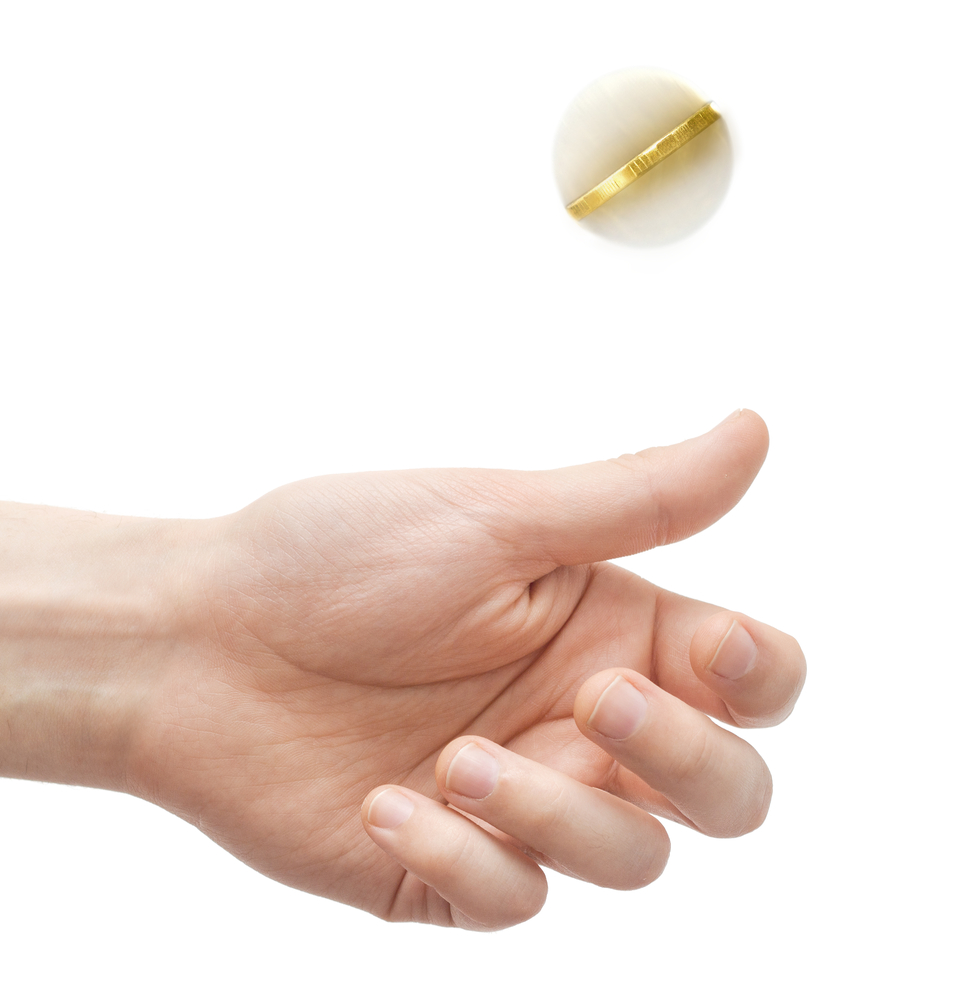
\includegraphics[height=0.5\textheight]{Coin-toss}
    \end{center}
\end{frame}

\begin{frame}
    \frametitle{Interpretación}
    \begin{block}{Frecuentista}
        \begin{itemize}
            \item Frecuencia relativa de un evento repetido infinitas veces.
            \item Esperamos que la moneda caiga la mitad de las veces cara.
        \end{itemize}
    \end{block}
    \begin{block}{Bayesiana / subjetiva}
        \begin{itemize}
            \item Incertidumbre sobre un evento.
            \item Relacionada con la información.
            \item Creemos podría caer tanto cara como cruz.
        \end{itemize}
    \end{block}
\end{frame}

\begin{frame}
    \frametitle{Interpretación}
    \begin{block}{Ejemplos: probabilidad de que...}
        \begin{itemize}
            \item Un paciente tenga COVID-19.
            \item Alguien de 68 años muera de cáncer fumando dos cajetillas diarias por 50 años.
            \item Un acusado de ser el asesino de su esposa, dada la evidencia.
            \item Los poemas escritos por Pablo Neruda hayan sido escritos por otro/a.
            \item Un mensaje en aula haya sido enviado por el/la estudiante.
        \end{itemize}
    \end{block}
    \begin{block}{Bayesiana / subjetiva}
        \begin{itemize}
            \item No se puede hacer inferencia sin supuestos.
            \item ¿Bondad o debilidad?
        \end{itemize}
    \end{block}
\end{frame}

\begin{frame}
    \frametitle{Recordar}
    \begin{block}{Probabilidades}
        \begin{itemize}
            \item ¿Dado un proceso que genera datos, cuáles son las propiedades que observaremos?
        \end{itemize}
    \end{block}
    \begin{center}
        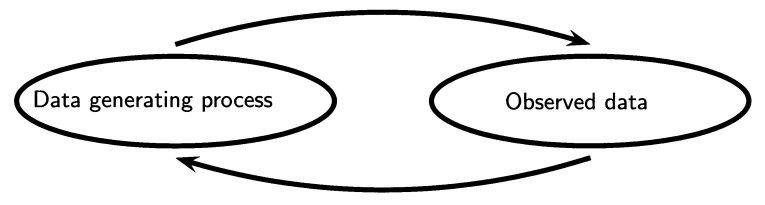
\includegraphics[height=0.3\textheight]{all2014_probabilidad_vs_inferencia}
    \end{center}
    \begin{block}{Inferencia estadística}
        \begin{itemize}
            \item ¿Dadas las observaciones, qué podemos decir sobre el proceso que genera los datos?
        \end{itemize}
    \end{block}
\end{frame}

\begin{frame}
    \frametitle{Ejemplo: moneda}
    \begin{tabular}{cc}
        50 repeticiones & 1000 repeticiones \\
        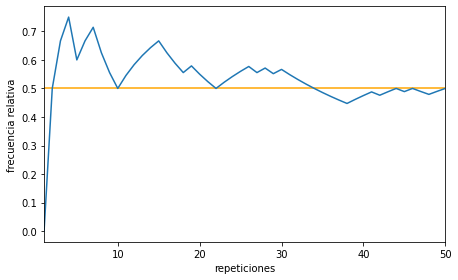
\includegraphics[width=0.49\textwidth]{moneda_50repeticiones} &
        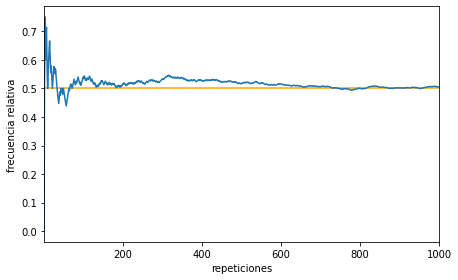
\includegraphics[width=0.49\textwidth]{moneda_1000repeticiones}
    \end{tabular}
\end{frame}

\iffalse
\begin{frame}
    \frametitle{Contando posibilidades: bolsa con 4 pelotas}
    \begin{block}{Posibilidades}
        \begin{center}
            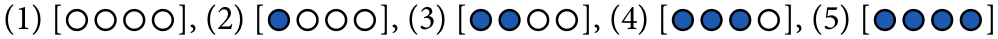
\includegraphics[height=0.05\textheight]{pelotas_todas}
        \end{center}
    \end{block}
    \begin{block}{Experimento}
        \begin{itemize}
            \item Se saca una pelota 3 veces con repetición:
        \end{itemize}
        \begin{center}
            
\includegraphics[height=0.05\textheight]{pelotas_datos}
        \end{center}
    \end{block}
    \begin{block}{Supuesto}
        \begin{center}
            
\includegraphics[height=0.05\textheight]{pelotas_conjetura}
        \end{center}
    \end{block}
\end{frame}

\begin{frame}
    \frametitle{Contando posibilidades: bolsa con 4 pelotas}
    \begin{center}
        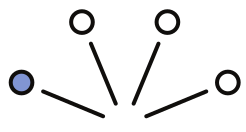
\includegraphics[height=0.2\textheight]{pelotas_arbol_1}
    \end{center}
\end{frame}

\begin{frame}
    \frametitle{Contando posibilidades: bolsa con 4 pelotas}
    \begin{center}
        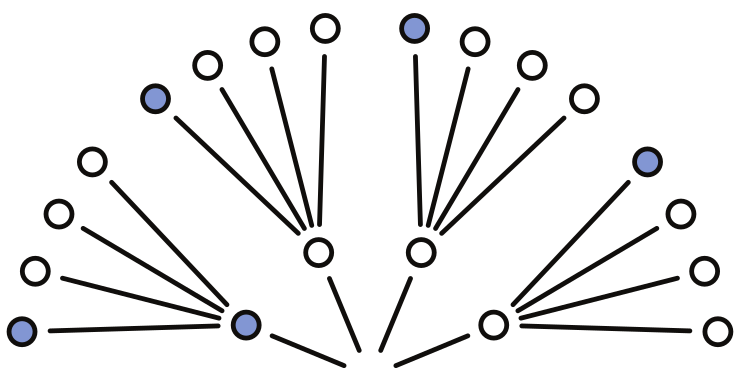
\includegraphics[height=0.5\textheight]{pelotas_arbol_2}
    \end{center}
\end{frame}

\begin{frame}
    \frametitle{Contando posibilidades: bolsa con 4 pelotas}
    \begin{center}
        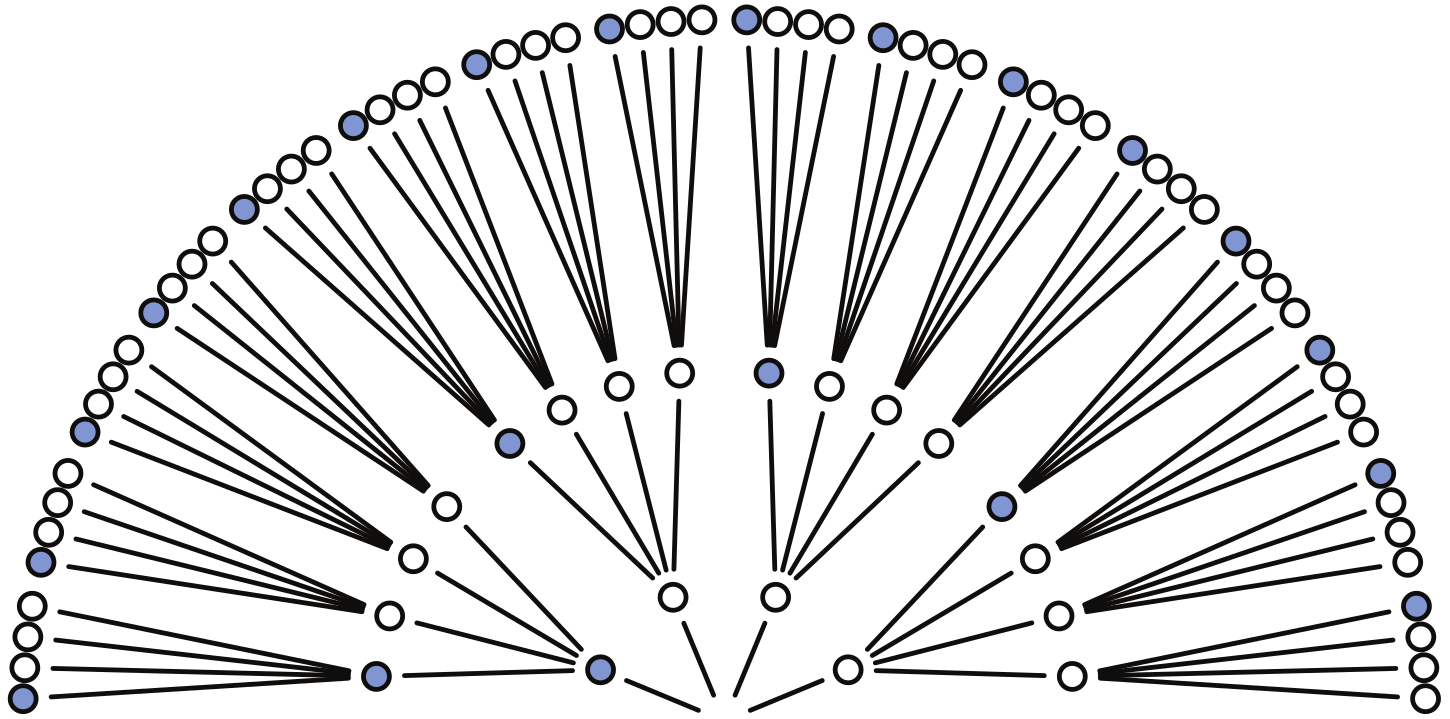
\includegraphics[height=0.5\textheight]{pelotas_arbol_3}
    \end{center}
\end{frame}

\begin{frame}
    \frametitle{Contando posibilidades: bolsa con 4 pelotas}
    \begin{center}
        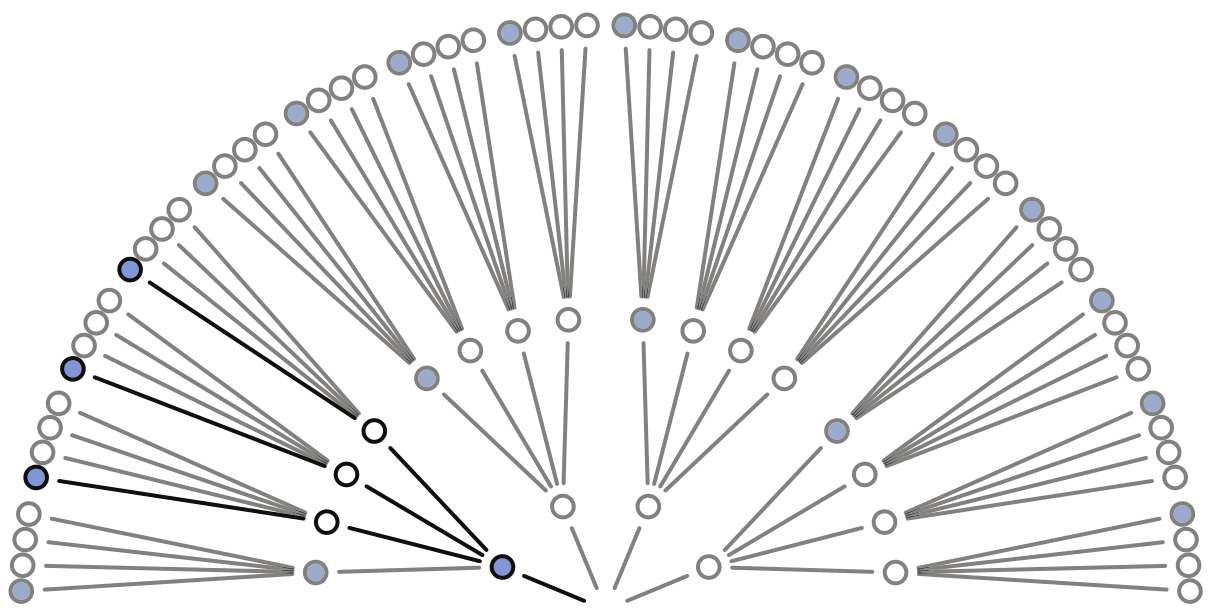
\includegraphics[height=0.513\textheight]{pelotas_arbol_4}
    \end{center}
\end{frame}

\begin{frame}
    \frametitle{Contando posibilidades: bolsa con 4 pelotas}
    \begin{center}
        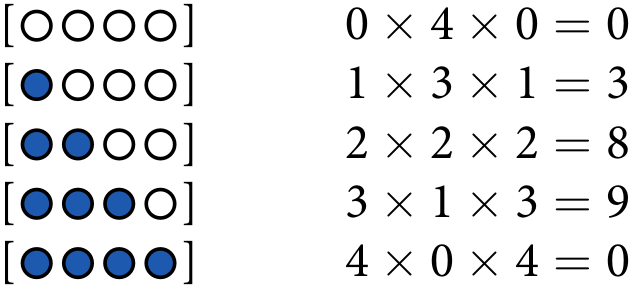
\includegraphics[height=0.4\textheight]{pelotas_conjeturas}
    \end{center}
\end{frame}
\fi

\begin{frame}
    \frametitle{Espacio muestral}
    \begin{block}{Espacio muestral ($\Omega$)}
        \begin{itemize}
            \item Conjunto de todos los posibles resultados de un \emph{experimento} aleatorio.
        \end{itemize}
    \end{block}
    \begin{block}{Ejemplos}
        \begin{itemize}
            \item Un dado: $\bparens{1 , 2 , 3 , 4 , 5 , 6}$.
            \item Una moneda: $\bparens{\text{cara} , \text{sello}}$.
            \item Dos lanzamientos de una moneda: $\bparens{\text{cc}, \text{cs}, \text{sc}, \text{ss}}$.
            \item En una carrera entre tres personas, posiciones de llegada: $\bparens{\parens{1, 2, 3}, \parens{1, 3, 2}, \parens{2, 1, 3}, \parens{2, 3, 1}, \parens{3, 1, 2}, \parens{3, 2, 1}}$.
            \item Ángulo en el que termina una ruleta $\sparens{0, 2 \pi}$.
        \end{itemize}
    \end{block}
\end{frame}

\begin{frame}
    \frametitle{Eventos}
    \begin{block}{Evento}
        \begin{itemize}
            \item Un subconjunto $A \subseteq \Omega$ del espacio muestral donde al final de un experimento podemos observar si el resultado $\omega \in \Omega$ está en $A$.
            \item $\bparens{\omega} \in \Omega$ evento simple o elemental.
            \item Más de un elemento: evento compuesto.
            \item $\Omega$ evento seguro.
            \item $\emptyset$ evento imposible o nulo.
        \end{itemize}
    \end{block}
    \begin{center}
        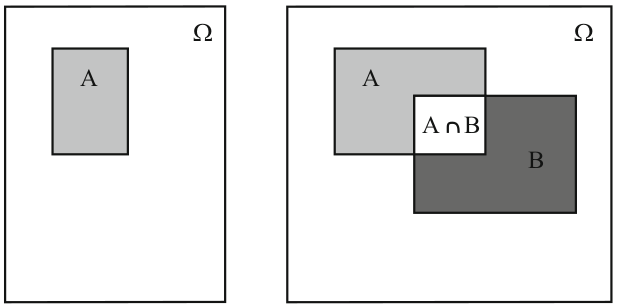
\includegraphics[width=0.6\textwidth]{diagrama_espacio_muestral_1}
    \end{center}
\end{frame}

\begin{frame}
    \frametitle{Eventos}
    \begin{block}{Ejemplo}
        \begin{itemize}
            \item Observar un número par al lanzar un dado:
                \begin{equation*}
                    A = \bparens{2, 4, 6} \subseteq \Omega = \bparens{1, 2, 3, 4, 5, 6}
                \end{equation*}
            \item Tiempo de vida de un componente electrónico sea menor que 5 años:
                \begin{equation*}
                    A = \bparens{t \in \reals \mid 0 < t < 5} \subseteq \Omega = \bparens{t \in \reals \mid t > 0}
                \end{equation*}
        \end{itemize}
    \end{block}
    \begin{center}
        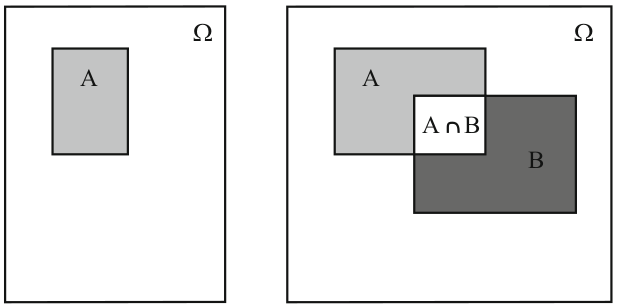
\includegraphics[width=0.6\textwidth]{diagrama_espacio_muestral_1}
    \end{center}
\end{frame}



%%%%%

\begin{frame}
    \frametitle{Eventos}

    \begin{block}{Ejercicio}

\begin{itemize}
\item Construya el espacio muestral para un experimento que consiste en lanzar un solo dado.
\item Encuentre los eventos que corresponden a las frases 'Se obtiene un numero par' y 'Se obtiene un numero mayor a 2'.
\end{itemize}

\end{block}

\end{frame}

\begin{frame}
    \frametitle{Eventos}

    \begin{block}{Ejercicio}
Un experimento aleatorio consiste en lanzar dos monedas al aire.
\begin{itemize}
\item Construya el espacio muestral para la situación en que las monedas son indistinguibles entre sí.
\item Construya el espacio muestral para la situación en que las monedas sí son distinguibles, por ejemplo de dos denominaciones distintas.
\end{itemize}

\end{block}

\end{frame}

\begin{frame}
    \frametitle{Eventos}

    \begin{block}{Ejercicio}
Construya el espacio muestral que describa  las posibles familias de 3 hijxs en terminos de los generos de estos individuos.

\end{block}

\end{frame}

%%%%

\begin{frame}
    \frametitle{Espacio de eventos ($\eventspace$)}
        \begin{itemize}
            \item Conjunto de todos los eventos $A$.
            \item Si $\Omega$ es finito, generalmente $\eventspace = 2^{\Omega}$.
        \end{itemize}
   \begin{block}{$\sigma$-álgebra}
        \begin{itemize}
				\item Colección de subconjuntos de $\Omega$
            \item Si $A \in \eventspace$, entonces $A^{c} \in \eventspace$.
            \item $\Omega \in \eventspace$.
            \item Si $\bparens{A_{i}}_{i \in I} = \bparens{A_{1}, A_{2}, \ldots, A_{i}, \ldots} \subseteq \eventspace$ es una colección finita o numerable de eventos, entonces $\bigcup_{i \in I} A_{i} \in \eventspace$.
        \end{itemize}
    \end{block}
\end{frame}

\begin{frame}
    \frametitle{Probabilidad ($P$)}
       \begin{itemize}
            \item Función $P: \eventspace \rightarrow \sparens{0, 1}$ que asocia un número a $A \in \eventspace$.
            \item Indica la probabilidad de obtener un resultado $\omega \in A$.
            \item Axiomas (Kolmogorov):
                \begin{itemize}
                    \item $\forall A \subseteq \eventspace, \prob{A} \geq 0$
                    \item $\prob{\Omega} = 1$.
                    \item Si $\bparens{A_{i}}_{i \in I} = \bparens{A_{1}, A_{2}, \ldots, A_{i}, \ldots} \subseteq \eventspace$ es una colección finita o numerable de eventos \emph{disjuntos} ($\forall A_{j}, A_{k} \in \bparens{A_{i}}_{i \in I}, A_{j} \cap A_{k} = \emptyset$), entonces $\prob{\bigcup_{i \in I} A_{i}} = \sum_{i \in I} \prob{A_{i}}$.
                \end{itemize}
        \end{itemize}

\end{frame}

\begin{frame}
    \frametitle{Ejemplos}
    \begin{block}{Proposición}
        \begin{itemize}
            \item $\prob{\emptyset} = 0$.
        \end{itemize}
    \end{block}
    \begin{block}{Demostración}
        \begin{itemize}
            \item Axiomas 2 y 3:
                \begin{equation*}
                    1 = \prob{\Omega} = \prob{\Omega \cup \emptyset} = \prob{\Omega} + \prob{\emptyset} = 1 + \prob{\emptyset} .
                \end{equation*}
        \end{itemize}
    \end{block}
    \begin{block}{Proposición}
        \begin{itemize}
            \item $\prob{A^{c}} = 1 - \prob{A}$.
        \end{itemize}
    \end{block}
    \begin{block}{Demostración}
        \begin{itemize}
            \item Axiomas 2 y 3:
                \begin{equation*}
                    1 = \prob{\Omega} = \prob{A \cup A^{c}} = \prob{A} + \prob{A^{c}} .
                \end{equation*}
        \end{itemize}
    \end{block}
\end{frame}

\begin{frame}
    \frametitle{Ejemplos}
    \begin{block}{Proposición}
        \begin{itemize}
            \item $\prob{A} \leq 1$.
        \end{itemize}
    \end{block}
    \begin{block}{Demostración}
        \begin{itemize}
            \item Axiomas 1, 2 y 3:
                \begin{equation*}
                    1 = \prob{\Omega} = \prob{A \cup A^{c}} = \prob{A} + \prob{A^{c}} \geq \prob{A} + 0 = \prob{A} .
                \end{equation*}
        \end{itemize}
    \end{block}
\end{frame}

\begin{frame}
    \frametitle{Ejemplos}
    \begin{block}{Proposición}
        \begin{itemize}
            \item $\prob{A \cup B} = \prob{A} + \prob{B} - \prob{A \cap B}$.
        \end{itemize}
    \end{block}
    \begin{center}
        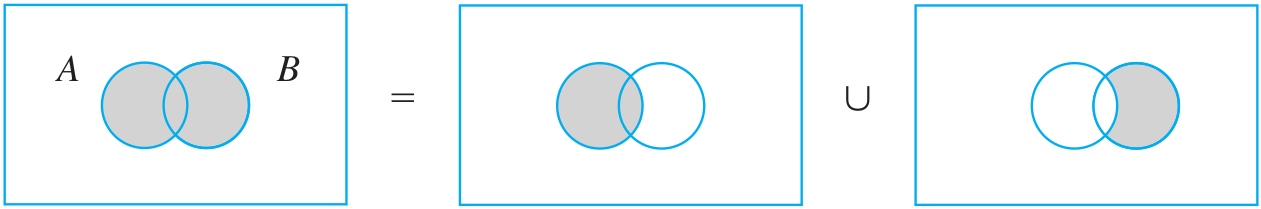
\includegraphics[width=0.9\textwidth]{venn_union}
    \end{center}
    \begin{block}{Demostración}
        \begin{itemize}
            \item Axioma 3:
                \begin{multline*}
                    \prob{A \cup B} = \prob{A \cup \parens{B \cap A^{c}}} = \prob{A} + \prob{B \cap A^{c}} ,
                    \\
                    \prob{B} = \prob{\parens{A \cap B} \cup \parens{B \cap A^{c}}} = \prob{A \cap B} + \prob{B \cap A^{c}}
                    \\
                    \Rightarrow \prob{A \cup B} = \prob{A} + \prob{B} - \prob{A \cap B} .
                \end{multline*}
        \end{itemize}
    \end{block}
\end{frame}



%%%%%%%%

\begin{frame}
    \frametitle{Probabilidad}

    \begin{block}{Ejercicio}
Un sistema compuesto por dos componentes A y B, se encuentra cableado de tal manera que pueda funcionar si cualquiera de los dos componentes también lo hace.
Se sabe por experimentos anteriores que P(A) es 0.9, P(B) es 0.8 y P(A y B) es 0.72.


Determine la probabilidad de que el sistema falle (i.e. No funcione).

\end{block}

\end{frame}

%%%%%%%%

\begin{frame}
    \frametitle{Relación teoría de conjuntos y teoría de probabilidades}
    \begin{center}
        \begin{tabular}{c|c|c}
            & Conjuntos & Eventos \\
            \hline
            $\Omega$ & Universo & Espacio Muestral \\
            $\mathcal{P} \parens{\Omega} = 2^{\Omega}$ & Conjunto potencia & Espacio de eventos (*finito) \\
            $A \subseteq \Omega$ & $A$ subconjunto de $\Omega$ & Evento $A$ \\
            $\omega \in A$ & Elemento $\omega$ & Resultado $\omega$ \\
            $\emptyset$ & Conjunto vacío & Evento imposible \\
            $\Omega$ & Universo & Evento seguro \\
            $A \cup B$ & $A$ unión $B$ & Evento $A$ o $B$ \\
            $A \cap B$ & $A$ intersección $B$ & Evento $A$ y $B$ \\
            $A^{c}$ & Complemento de $A$ & Evento no $A$, opuesto de $A$ \\
            $A \subseteq B$ & $A$ subconjunto de $B$ & $A$ implica $B$ \\
            $A \cap B = \emptyset$ & $A$ y $B$ disjuntos & $A$ y $B$ mutuamente excluyentes \\
        \end{tabular}
    \end{center}
\end{frame}

\begin{frame}
    \frametitle{Preguntas}
    \begin{exampleblock}{Propiedades básicas}
        Sean $A$ y $B$ eventos tales que $\prob{A} = \alpha$ y $\prob{B} = \beta$.
        \begin{enumerate}
            \item Acote $\prob{A \cap B}$ y $\prob{A \cup B}$ inferior y superiormente.
            \item Si $\prob{A \cap B} = \gamma$, escriba las siguientes expresiones en función de $\alpha$, $\beta$ y $\gamma$:
                \begin{enumerate}
                    \item $\prob{A^{C} \cup B^{C}}$.
                    \item $\prob{A^{C} \cap B}$.
                    \item $\prob{A^{C} \cup B}$.
                    \item $\prob{A^{C} \cap B^{C}}$.
                \end{enumerate}
        \end{enumerate}
    \end{exampleblock}
\end{frame}

\begin{frame}
    \begin{center}
        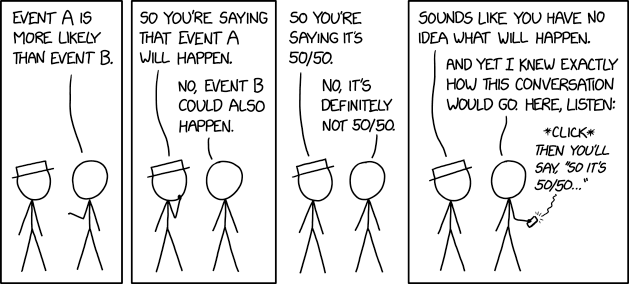
\includegraphics[height=0.5\textheight]{xkcd_prediction}
    \end{center}
\end{frame}

\begin{frame}
    \frametitle{¿Cómo se define el valor?}
    \begin{block}{Eventos equiprobables (Laplace)}
        \begin{itemize}
            \item Si $\Omega$ es finito y cada evento es igual de probable:
                \begin{multline*}
                    1 = \prob{\Omega} = \prob{\bigcup_{i = 1}^{n} \bparens{\omega_{i}}} = \sum_{i = 1}^{n} \prob{\bparens{\omega_{i}}} = n \prob{\bparens{\omega_{1}}} = n p
                    \\
                    \Rightarrow p = \prob{\bparens{\omega_{i}}} = \frac{1}{n} = \frac{1}{\vparens{\Omega}} .
                \end{multline*}
            \item De la misma manera:
                \begin{equation*}
                    \prob{A} = \prob{\bigcup_{i = 1}^{n_{A}} \bparens{\omega_{i}}} = \sum_{i = 1}^{n_{A}} \prob{\bparens{\omega_{i}}} = n_{A} p = \frac{n_{A}}{n} = \frac{\vparens{A}}{\vparens{\Omega}}
                \end{equation*}
        \end{itemize}
    \end{block}
\end{frame}

\begin{frame}
	 \begin{block}{Composición de una Escuela}
		El cuerpo de estudiantes de una escuela se compone según raza y etnia de la siguiente manera: 51\% blanca, 27\% negra, 11\% hispana, 6\% asiática y 5\% de otras. Se selecciona un estudiante al azar de esta escuela. Encuentre las probabilidades de los siguientes eventos:
	\begin{itemize}
		\item B : El/las estudiante es de raza negra.
		\item M: El/estudiante no es blanca (i.e. Es una minoría).
		\item N: El/la estudiante no es de raza negra.
	\end{itemize}

    \end{block}
\end{frame}


\begin{frame}
	 \begin{block}{Composición de una otra Escuela}
		El cuerpo de estudiantes de otra escuela está compuesto por 10 grupos según raza y etnia: 25\% de hombres de raza blanca, 26\% de mujeres de la misma raza, 12\% de hombres de raza negra, 15\% de mujeres de raza negra, 6\% de hombres hispanos, 5\% de mujeres hispanas, 3\% de hombres asiaticos, 3\% de mujeres asiaticas, 1\% de hombres de otras razas minoritarias, y 4\% de mujeres de estas mismas razas combinadas.
Se selecciona un estudiante al azar de esta escuela.
Encuentre las probabilidades de los siguientes eventos:
	\begin{itemize}
		\item B : La/el estudiante es de raza negra.
		\item MF: La estudiante es una mujer de una minoría.
		\item FN: La estudiante es una mujer y no es de raza negra.
	\end{itemize}

    \end{block}
\end{frame}


\begin{frame}
    \frametitle{Técnicas de conteo}

	\begin{block}{Teorema fundamental del Conteo}
		Si una tarea consiste de $k$ sub-tareas individuales, de las cuales la i-ésima puede ser realizada de $n_i$ maneras ($i= 1,\ldots ,k$), entonces la tarea completa puede ser realizada  de $n_1\times n_2\times \ldots n_k$ maneras distintas. 
	\end{block}
	
\end{frame}



\begin{frame}
    \frametitle{Técnicas de conteo}

	\begin{block}{Ejemplo - Teorema fundamental del Conteo}
		En un concurso de lotería se dispone de 44 números ($1\ldots 44$), de los cuales cada participante deberá escoger $6$ (sin repetición). El billete ganador será generado finalmente escogiendo al azar 6 números.

	Para poder calcular la probabilidad de tener el billete ganador, primero tendremos que calcular cuantos grupos de 6 números pueden ser escogidos.
		
	\end{block}
	\pause
\textbf{¿Como cambia el cálculo anterior si ahora escoger el mismo número varias veces?}

\end{frame}


\begin{frame}
    \frametitle{Técnicas de conteo}
	En ocasiones al contar, debemos contar objetos en un orden particular y en otras este orden no es relevante.
		\begin{itemize}
		\item Existen 5 candidatos en una elección. Suponiendo que no hay empates, ¿de cuantas formas pueden ocuparse los primeros 3 lugares?
		\begin{itemize}
			\item Es importante quien ocupa cada lugar.
		\end{itemize}

		\item Un periodista visita un curso de 25 estudiantes para entrevistar a 4 ¿De cuantas maneras se pueden escoger los 4 estudiantes?
		\begin{itemize}
			\item A quien se entrevista primero no es relevante.
		\end{itemize}

		\end{itemize}

\end{frame}


\begin{frame}
    \frametitle{Técnicas de conteo}

		A los arreglos ordenados se les llama \textbf{permutaciones} y a los sin orden, \textbf{combinaciones}.

\begin{table}[]
\begin{tabular}{lll}
        & \multicolumn{1}{c}{\begin{tabular}[c]{@{}c@{}}Sin \\ reemplazo\end{tabular}} & \multicolumn{1}{c}{\begin{tabular}[c]{@{}c@{}}Con\\ reemplazo\end{tabular}} \\
C/Orden & $\frac{n!}{(n-k)!}$                                                          & $n^k$                                                                       \\
S/Orden & $\binom{n}{k}$                                                               & $\binom{n+k-1}{k}$                                                         
\end{tabular}
\end{table}


Estos mecanismos de conteo son útiles cuando el espacio muestral es finito y todos sus resultados equiprobables.

\end{frame}



\begin{frame}
    \frametitle{Técnicas de conteo}

	\begin{itemize}
		\item Por lo tanto, para un espacio $S$ con $N$ resultados implica que $P(\{s_i\})=\frac{1}{N}$
		\item $$ P(A)=\sum_{s_i\in A}P(\{s_i\})= \sum_{s_i\in A}\frac{1}{N} =\frac{\#\mbox{ elementos en A}}{\#\mbox{ elementos en S}}$$
		\item Las estrategias de conteo pueden ser usadas para calcular tanto las expresiones del numerador como del denominador.
	\end{itemize}

\end{frame}


\begin{frame}
    \frametitle{Problemas de conteo}
		Considere una mano de pocker de 5 cartas tomadas desde un deck standard de 52 cartas. 
		\begin{itemize}
			\item No hay reemplazo y el orden no es relevante
			\item ¿Cual es el espacio muestral?

			\item ¿Cual es el total de manos de 5 cartas?

			\item ¿Cual es la probabilidad de tener una mano con 4 aces?
		\end{itemize}

  \begin{tikzpicture}[remember picture, overlay]
    \node[above=1.0cm] at (current page.south) 
    {
        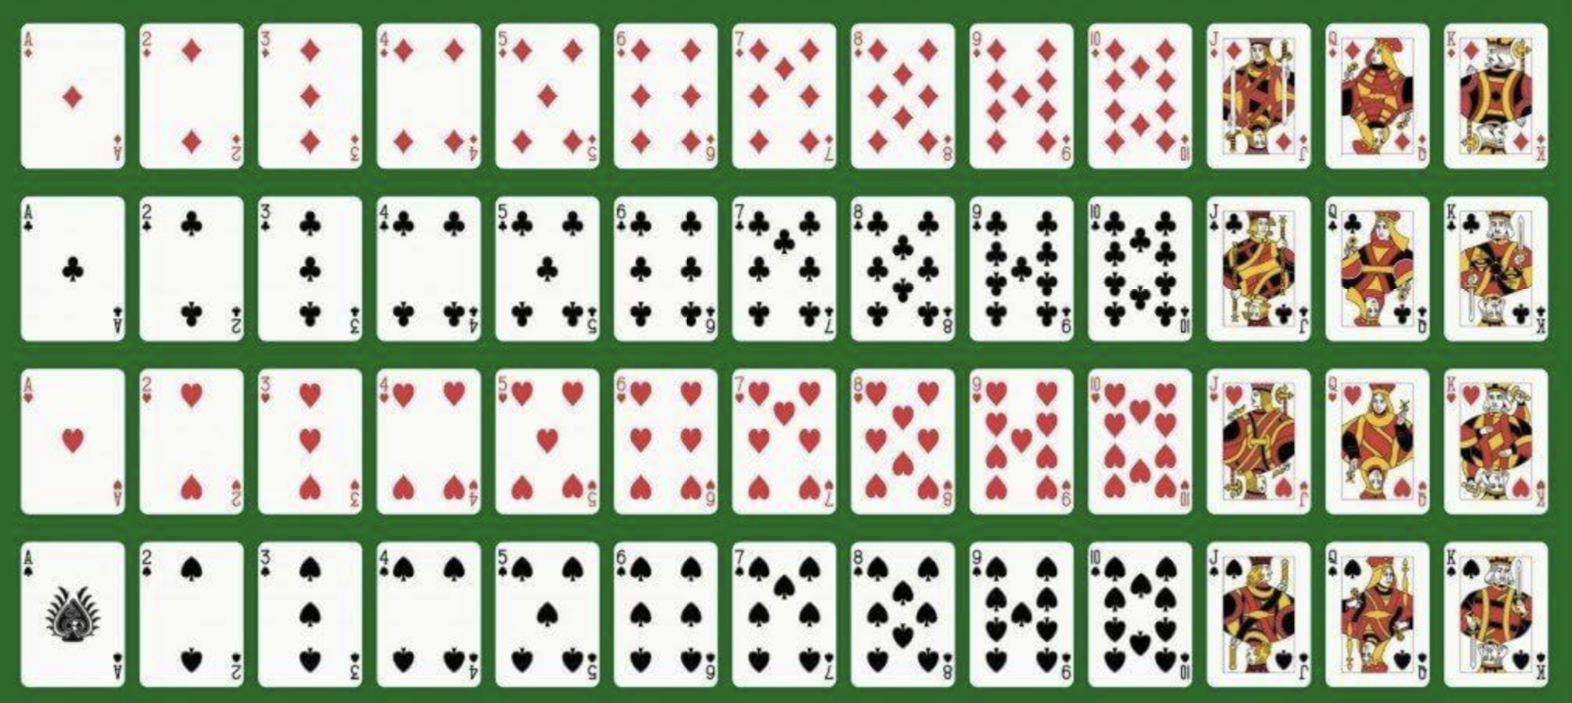
\includegraphics[width=0.4\textwidth]{deck52.png}
    };
  \end{tikzpicture}

\end{frame}


\begin{frame}
    \frametitle{Problemas de conteo}
		Considere una mano de pocker de 5 cartas tomadas desde un deck standard de 52 cartas. 

		\begin{itemize}
			\item ¿Cual es la probabilidad de obtener 4 cartas del mismo tipo?
			\item ¿...de tener exactamente un par?
		\end{itemize}

	\begin{tikzpicture}[remember picture, overlay]
    \node[above=1.0cm, xshift=4cm, yshift=1cm] at (current page.south) 
    {
        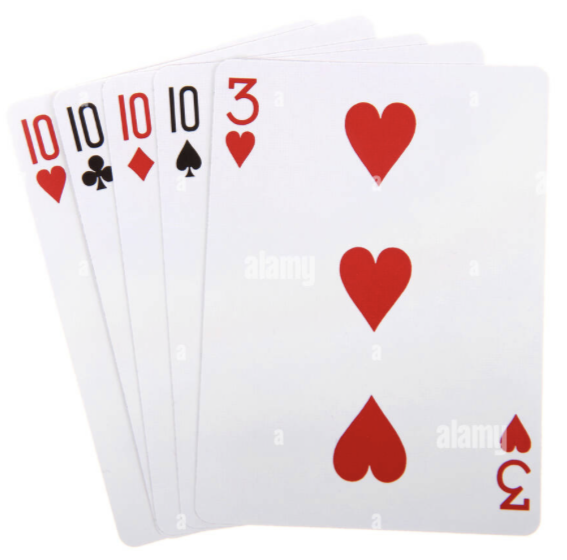
\includegraphics[width=0.23\textwidth]{four-of-a-kind.png}
    };
  \end{tikzpicture}

	\begin{tikzpicture}[remember picture, overlay]
    \node[above=1.0cm, xshift=-1cm, yshift=1cm] at (current page.south) 
    {
        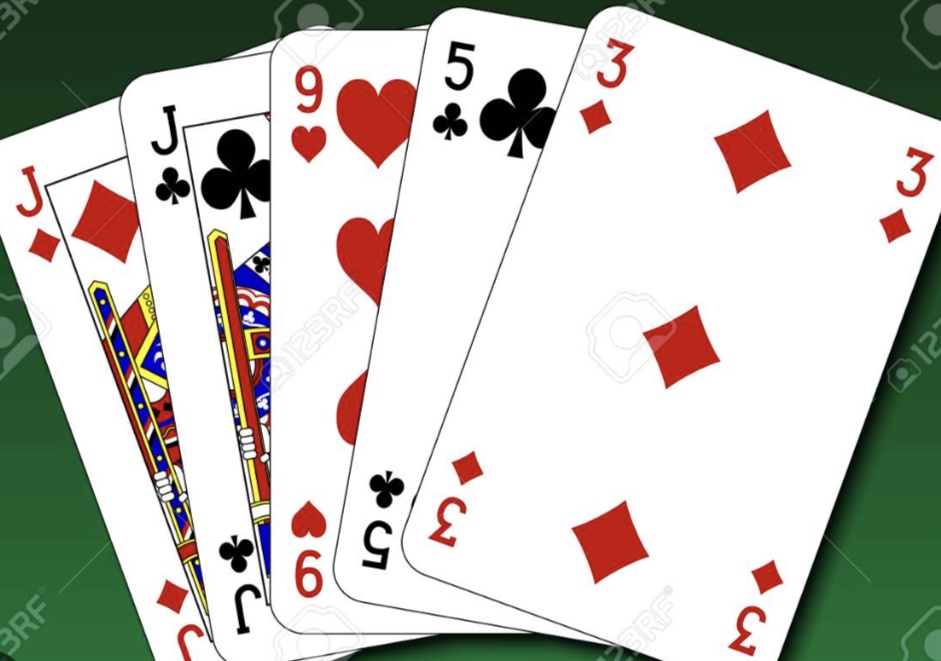
\includegraphics[width=0.26\textwidth]{single-pair-hand.png}
    };
  \end{tikzpicture}

\end{frame}
%%%%%%%%%%% %%%%%%%%%%% %%%%%%%%%%% 
\iffalse

\begin{frame}
    \frametitle{Técnicas de conteo}
    \begin{block}{Pares ordenados}
        \begin{itemize}
            \item Un elemento de conjunto finito $\Omega_{1}$ y segundo de conjunto finito $\Omega_{2}$.
            \item $\Omega = \Omega_{1} \times \Omega_{2}$.
            \item $\vparens{\Omega} = \vparens{\Omega_{1}} \vparens{\Omega_{2}}$.
            \item Si $\Omega_{1} = \Omega_{2}$, entonces $\vparens{\Omega} = \vparens{\Omega_{1}}^{2}$.
            \item En general, si $\Omega = \Omega_{1} \times \ldots \times \Omega_{k}$, entonces
                $\vparens{\Omega} = \vparens{\Omega_{1}} \cdots \vparens{\Omega_{k}}$.
        \end{itemize}
    \end{block}
    \begin{center}
        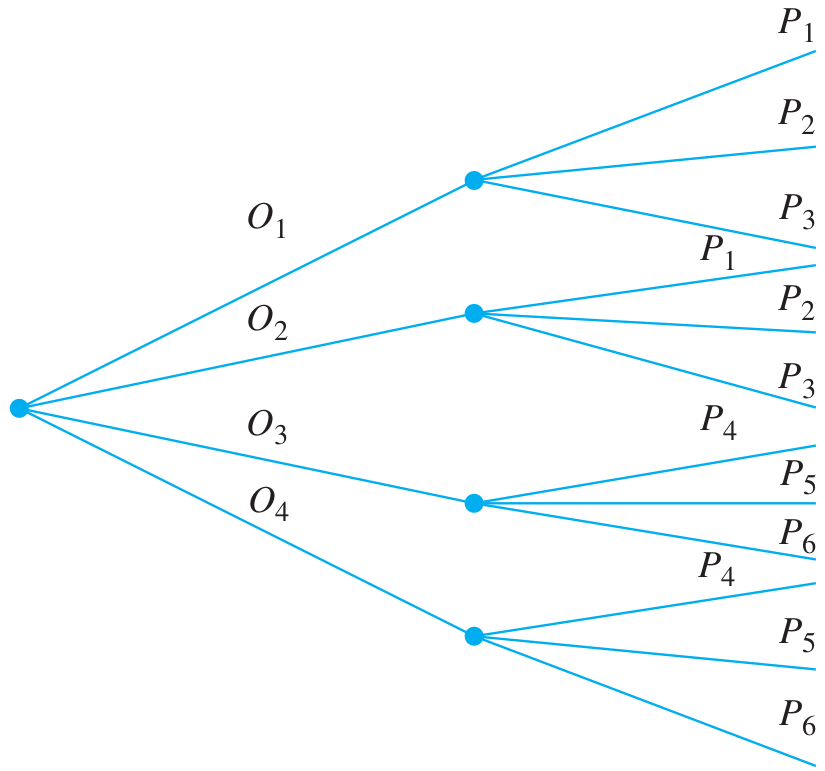
\includegraphics[width=0.4\textwidth]{arbol_producto}
    \end{center}
\end{frame}

\begin{frame}
    \frametitle{Ejemplos}
    \begin{block}{String de 20 bytes}
        \begin{itemize}
            \item Probabilidad de adivinar un string de 20 bytes.
        \end{itemize}
    \end{block}
\end{frame}

\begin{frame}
    \frametitle{Ejemplos}
    \begin{block}{Ruido}
        \begin{itemize}
            \item Escribo número binario de 10 bits tirando una moneda para cada bit.
            \item Si moneda sale cara, escribo el bit correcto, sino, el contrario.
            \item Probabilidad de escribir el número correcto.
        \end{itemize}
    \end{block}
\end{frame}

\begin{frame}
    \frametitle{Ejemplos}
    \begin{block}{Número}
        \begin{itemize}
            \item Pienso en un número entre 0 y 1024.
            \item Probabilidad de que el número sea divisible por 32.
        \end{itemize}
    \end{block}
\end{frame}

\begin{frame}
    \frametitle{Ejemplos}
    \begin{block}{Colores}
        \begin{itemize}
            \item Tengo 3 camisas de colores diferentes (azul, rojo, verde).
            \item Tengo 2 pantalones de colores diferentes (negro, azul).
            \item Probabilidad de usar camisa y pantalón del mismo color.
        \end{itemize}
    \end{block}
\end{frame}

\begin{frame}
    \frametitle{Ejemplos}
    \begin{block}{Colores 2}
        \begin{itemize}
            \item Tengo 3 camisas de colores diferentes (azul, negro, verde).
            \item Tengo 2 pantalones de colores diferentes (negro, azul).
            \item Probabilidad de usar camisa y pantalón del mismo color.
        \end{itemize}
    \end{block}
\end{frame}

\begin{frame}
    \frametitle{Técnicas de conteo}
    \begin{block}{Permutaciones}
        \begin{itemize}
            \item Subconjunto, selección ``ordenada'' de tamaño $k$ de conjunto de tamaño $n$:
                \begin{equation*}
                    \frac{n !}{\parens{n - k} !} .
                \end{equation*}
        \end{itemize}
    \end{block}
\end{frame}

\begin{frame}
    \frametitle{Ejemplos}
    \begin{block}{Lugares}
        \begin{itemize}
            \item Un curso tiene 50 estudiantes (Ana, Bernardo, Cristián, Daniela, etc.).
            \item 20 de ellos llegan a la clase.
            \item Probabilidad de que la primera en llegar sea Ana y el último Cristián.
        \end{itemize}
    \end{block}
\end{frame}

\begin{frame}
    \frametitle{Técnicas de conteo}
    \begin{block}{Combinaciones}
        \begin{itemize}
            \item Subconjunto, selección ``desordenada'' de tamaño $k$ de conjunto de tamaño $n$:
                \begin{equation*}
                    \begin{pmatrix}
                        n \\ k
                    \end{pmatrix}
                    = \frac{n !}{\parens{n - k} ! k !} .
                \end{equation*}
            \item Recordar:
                \begin{equation*}
                    \sum_{i = 0}^{n} \combin{n}{i} = 2^{n} .
                \end{equation*}
        \end{itemize}
    \end{block}
    \begin{block}{Nota: aproximación de Stirling}
        \begin{itemize}
            \item $x ! \approx x^{x} e^{- x} \sqrt{2 \pi x}$.
            \item $\ln \parens{x !} \approx x \ln \parens{x} - x + \frac{1}{2} \ln \parens{2 \pi x}$.
        \end{itemize}
    \end{block}
\end{frame}

\begin{frame}
    \frametitle{Ejemplos}
    \begin{block}{Juego de azar}
        \begin{itemize}
            \item Probabilidad de ganar el kino (14 números entre 25).
            \item Probabilidad de ganar el loto (6 números entre 41).
        \end{itemize}
    \end{block}
\end{frame}

\begin{frame}
    \frametitle{Ejemplos}
    \begin{block}{Grupos}
        \begin{itemize}
            \item Un curso tiene 50 estudiantes (Ana, Bernardo, Cristián, Daniela, etc.).
            \item Selección aleatoria de 3 estudiantes para participar en competencia.
            \item Probabilidad de que el grupo contenga a Ana.
        \end{itemize}
    \end{block}
\end{frame}

\begin{frame}
    \frametitle{Ejemplos}
    \begin{block}{Selección de películas}
        \begin{itemize}
            \item Dos personas ven 3 películas de entre 100 en un festival de cine.
            \item Probabilidad de que ambas hayan visto las mismas 3 películas.
        \end{itemize}
    \end{block}
\end{frame}

\begin{frame}
    \frametitle{Ejemplos}
    \begin{block}{Paradoja del cumpleaños}
        \begin{itemize}
            \item 50 personas ven 1 película de entre 100 en un festival de cine.
            \item Probabilidad de que al menos dos hayan visto la misma película.
        \end{itemize}
    \end{block}
\end{frame}

\begin{frame}
    \frametitle{Probabilidad condicional}
    \begin{block}{Definición}
        \begin{itemize}
            \item Sean $A$ y $B$ dos eventos, tal que $\prob{B} > 0$:
        \end{itemize}
        \begin{equation*}
            \prob{A \mid B} = \frac{\prob{A \cap B}}{\prob{B}} = \frac{\prob{A, B}}{\prob{B}} .
        \end{equation*}
    \end{block}
    \begin{block}{Interpretación}
        \begin{itemize}
            \item Si ocurre $B$, ¿cuál es la probabilidad de $A$?
            \item $B$ se transforma en el nuevo espacio muestral.
        \end{itemize}
    \end{block}
    \begin{center}
        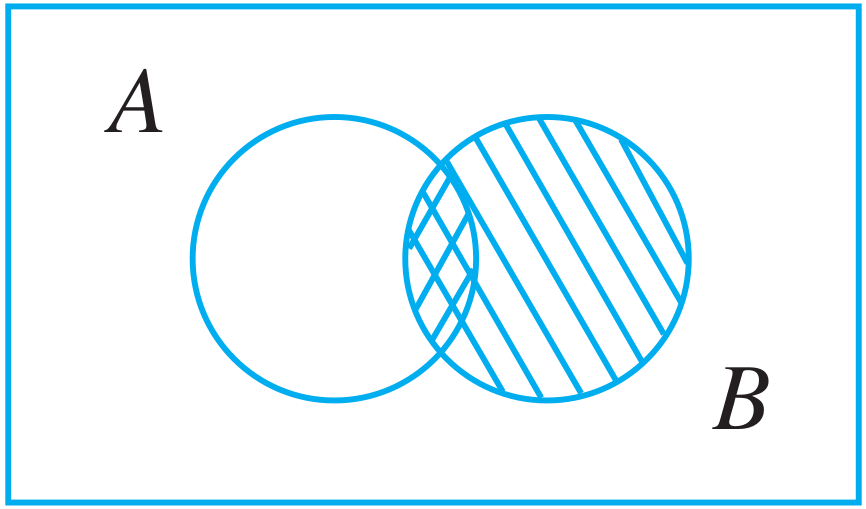
\includegraphics[width=0.4\textwidth]{venn_condicional}
    \end{center}
\end{frame}

\begin{frame}
    \frametitle{Probabilidad condicional}
    \begin{exampleblock}{Ejemplo: lanzamiento de dado}
        \begin{itemize}
            \item Probabilidad de obtener resultado 3, si sé que el resultado es impar.
            \item Probabilidad de obtener resultado 3, si sé que el resultado es par.
        \end{itemize}
    \end{exampleblock}
\end{frame}
\fi
%%%%%%%%%%%%%%%



\begin{frame}
    \frametitle{Probabilidad condicional}
    \begin{exampleblock}{Ejemplo: g\'enero de reci\'en nacido/a}
        \begin{itemize}
            \item Juan tiene dos hijos o hijas. La mayor es una chica, ¿Probabilidad de que ambas sean chicas?
            \item Mar\'ia tiene dos hijas o hijos. Una de ellas es chica. ¿Probabilidad de que ambas sean chicas?
        \end{itemize}
    \end{exampleblock}
\end{frame}

\begin{frame}
    \frametitle{Probabilidad condicional}
    \begin{block}{Ejemplo: examen}
        \begin{itemize}
            \item Probabilidad de examen positivo, si tiene enfermedad.
            \item Probabilidad de examen positivo, si no tiene enfermedad.
        \end{itemize}
    \end{block}
    \begin{center}
        \begin{tabular}{c|cc}
            & Enfermedad & No Enfermedad \\
            \hline
            Examen Positivo & 290 & 10000 \\
            Examen Negativo & 10 & 200000 \\
        \end{tabular}
    \end{center}
\end{frame}

\begin{frame}
    \frametitle{Probabilidad condicional}
    \begin{block}{Ejemplo: examen}
        \begin{itemize}
            \item Probabilidad de tener enfermedad, si examen es positivo.
            \item Probabilidad de tener enfermedad, si examen es negativo.
        \end{itemize}
    \end{block}
    \begin{center}
        \begin{tabular}{c|cc}
            & Enfermedad & No Enfermedad \\
            \hline
            Examen Positivo & 290 & 10000 \\
            Examen Negativo & 10 & 200000 \\
        \end{tabular}
    \end{center}
\end{frame}

\begin{frame}
    \frametitle{Probabilidad condicional}
    \begin{center}
        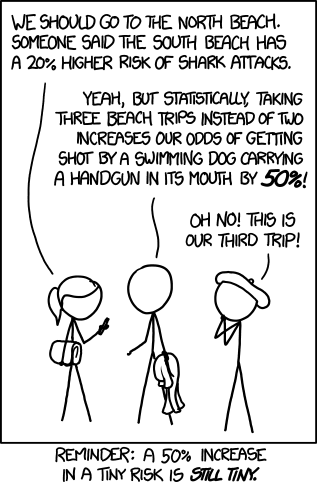
\includegraphics[height=0.8\textheight]{xkcd_increased_risk}
    \end{center}
\end{frame}

\begin{frame}
    \frametitle{Independencia}
    \begin{block}{Definición}
        \begin{itemize}
            \item Sean $A$ y $B$ dos eventos. Son independientes si y solo si:
                \begin{equation*}
                    \prob{A \mid B} = \prob{A} .
                \end{equation*}
            \item Equivale a:
                \begin{equation*}
                    \prob{A, B} = \prob{A} \prob{B} .
                \end{equation*}
        \end{itemize}
    \end{block}
    \begin{block}{Interpretación}
        \begin{itemize}
            \item Conocer parte de un resultado no nos dice nada del otro.
            \item Conocer $B$ no tiene efecto en la probabilidad de $A$.
        \end{itemize}
    \end{block}
\end{frame}

\begin{frame}
    \frametitle{Independencia}
    \begin{block}{Ejemplo: lanzamiento de dados}
        \begin{itemize}
            \item Probabilidad de que el segundo dado sea par, si el primero es 3.
            \item Probabilidad de que el segundo dado sea par, si el primero es impar.
        \end{itemize}
    \end{block}
    \begin{center}
        \begin{tabular}{c|cccccc}
            $\Omega$ & 1 & 2 & 3 & 4 & 5 & 6 \\
            \hline
            1 & $\parens{1, 1}$ & $\parens{1, 2}$ & $\parens{1, 3}$ & $\parens{1, 4}$ & $\parens{1, 5}$ & $\parens{1, 6}$ \\
            2 & $\parens{2, 1}$ & $\parens{2, 2}$ & $\parens{2, 3}$ & $\parens{2, 4}$ & $\parens{2, 5}$ & $\parens{2, 6}$ \\
            3 & $\parens{3, 1}$ & $\parens{3, 2}$ & $\parens{3, 3}$ & $\parens{3, 4}$ & $\parens{3, 5}$ & $\parens{3, 6}$ \\
            4 & $\parens{4, 1}$ & $\parens{4, 2}$ & $\parens{4, 3}$ & $\parens{4, 4}$ & $\parens{4, 5}$ & $\parens{4, 6}$ \\
            5 & $\parens{5, 1}$ & $\parens{5, 2}$ & $\parens{5, 3}$ & $\parens{5, 4}$ & $\parens{5, 5}$ & $\parens{5, 6}$ \\
            6 & $\parens{6, 1}$ & $\parens{6, 2}$ & $\parens{6, 3}$ & $\parens{6, 4}$ & $\parens{6, 5}$ & $\parens{6, 6}$ \\
        \end{tabular}
    \end{center}
\end{frame}

\begin{frame}
%Falta la definicion de indenpendencia.
%Falta ejemplo en que la definicion de a pares no funciona.
\frametitle{Independencia}
\begin{block}{Ejemplo: Lanzamiento de un par de dados}
    \begin{itemize}
        \item Sea $A_1$ el evento en que el primer dado arroja un número impar.
        \item Sea $A_2$ el evento en que el segundo dado arroja un número impar.
        \item Sea $A_3$ el evento en que la suma de ambos dados es impar.
    \end{itemize}
\end{block}
\end{frame}

\begin{frame}
%Falta la definicion de indenpendencia.
%Falta ejemplo en que la definicion de a pares no funciona.
\frametitle{Independencia}
\begin{block}{Ejemplo: Lanzamiento de un par de dados}
    \begin{itemize}
        \item $A_1$ y $A_2$ son independientes con probabilidades: $$\prob{A_1}=\frac{1}{2},\ \prob{A_2}=\frac{1}{2}$$
        \item Adicionalmente $\prob{A_3}=\frac{18}{36}=\frac{1}{2}$
        \item Dado que $A_1$ ocurrió, $A_3$ puede ocurrir solo si el segundo dado arroja un número par $\Rightarrow$ $\prob{A_3|A_1}=\dfrac{9}{18}=\dfrac{1}{2}$
        \item Ídem para $\prob{A_3|A_2}$
    \end{itemize}
\end{block}
\end{frame}

\begin{frame}
%Falta la definicion de indenpendencia.
%Falta ejemplo en que la definicion de a pares no funciona.
\frametitle{Independencia}
\begin{block}{Ejemplo: Lanzamiento de un par de dados}
    \begin{itemize}
        \item Luego, $\prob{A_3|A_1}=\prob{A_3}$, $\prob{A_3|A_2}=\prob{A_3}$
        \item Por lo tanto, los eventos $A_1$ y $A_2$ son independientes, así como tambien lo son los eventos $A_2$ y $A_3$
    \end{itemize}
\end{block}
¿Que ocurre con $\prob{A_1,A_2,A_3}$?
\pause

$A_3$ no puede ocurrir si $A_1$ y $A_2$ ocurren simultáneamente. Es decir, $$\prob{A_1,A_2,A_3}=0$$

entonces $$\prob{A_1,A_2,A_3}\neq \prob{A_1}\prob{A_2}\prob{A_3}$$
\end{frame}


\begin{frame}
    \frametitle{Independencia generalización}
    \begin{block}{Definición}
        \begin{itemize}
            \item Los eventos $A_1,A_2,\ldots ,A_n$ son independientes (mutuamente) si:
                $$\prob{A_i, A_j} = \prob{A_i} \prob{A_j},$$
                $$\prob{A_i, A_j, A_k} = \prob{A_i} \prob{A_j} \prob{A_k},$$
                $$\ldots$$
                $$\prob{A_1,A_2,\ldots ,A_n}=\prob{A_1} \prob{A_2}\ldots \prob{A_n}$$
            \item Para todas las combinaciones de índices tales que $i\neq j\neq k\in [1\ldots n]$
        \end{itemize}
    \end{block}
\end{frame}

\begin{frame}
    \frametitle{Regla del producto}
    \begin{block}{Otra manera de escribir probabilidad condicional}
        \begin{itemize}
            \item Sean $A$ y $B$ dos eventos:
                \begin{equation*}
                    \prob{A, B} = \prob{A \cap B} = \prob{A \mid B} \prob{B} = \prob{B \mid A} \prob{A} .
                \end{equation*}
            \item Sea $\bparens{A_{1}, \ldots , A_{i}, \ldots, A_{n}}$ familia de eventos:
                \begin{multline*}
                    \prob{A_{1}, \ldots , A_{n}}
                    = \prob{A_{1} \mid A_{2} , \ldots, A_{n}} \prob{A_{2}, \ldots, A_{n}}
                    \\
                    = \prob{A_{1} \mid A_{2} , \ldots, A_{n}} \prob{A_{2} \mid A_{3}, \ldots, A_{n}} \prob{A_{3} , \ldots, A_{n}}
                    \\
                    \vdots
                    \\
                    = \prob{A_{n}} \prod_{i = 1}^{n - 1} \prob{A_{i} \mid A_{i + 1} , \ldots, A_{n}}.
                \end{multline*}
        \end{itemize}
    \end{block}
\end{frame}

\begin{frame}
    \frametitle{Ley de probabilidad total}
    \begin{block}{Eventos disjuntos / partición}
        \begin{itemize}
            \item $\bparens{B_{1}, \ldots, B_{n}}$ familia de eventos.
            \item Eventos disjuntos o mutuamente excluyentes: $\forall i, j, B_{i} \cap B_{j} = \emptyset$.
            \item Partición: disjuntos y $\bigcup_{i = 1}^{n} B_{i} = \Omega$.
        \end{itemize}
    \end{block}
    \begin{block}{Ley de probabilidad total}
        \begin{itemize}
            \item Sea $\bparens{B_{1}, \ldots, B_{n}}$ partición de $\Omega$:
                \begin{equation*}
                    \prob{A} = \sum_{i = 1}^{n} \prob{A \mid B_{i}} \prob{B_{i}} .
                \end{equation*}
        \end{itemize}
    \end{block}
    \begin{center}
        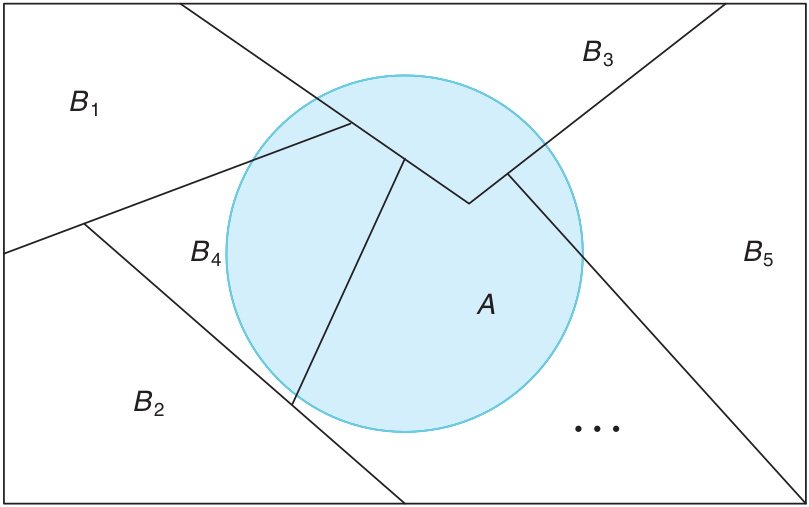
\includegraphics[width=0.35\textwidth]{venn_probabilidad_total}
    \end{center}
\end{frame}

\begin{frame}
    \frametitle{Regla / Teorema de Bayes}
    \begin{block}{Dos eventos}
        \begin{itemize}
            \item Sean $A$ y $B$ dos eventos:
                \begin{equation*}
                    \prob{B \mid A} = \frac{\prob{A \mid B} \prob{B}}{\prob{A}} .
                \end{equation*}
        \end{itemize}
    \end{block}
    \begin{block}{Eventos disjuntos}
        \begin{itemize}
            \item Sea $A$ un evento y $\bparens{B_{1}, \ldots, B_{n}}$ partición de $\Omega$:
                \begin{equation*}
                    \forall i, \prob{B_{i} \mid A} = \frac{\prob{A \mid B_{i}} \prob{B_{i}}}{\prob{A}}
                    =
                    \frac{\prob{A \mid B_{i}} \prob{B_{i}}}{\sum_{j = 1}^{n} \prob{A \mid B_{j}} \prob{B_{j}}} .
                \end{equation*}
        \end{itemize}
    \end{block}
    \begin{center}
        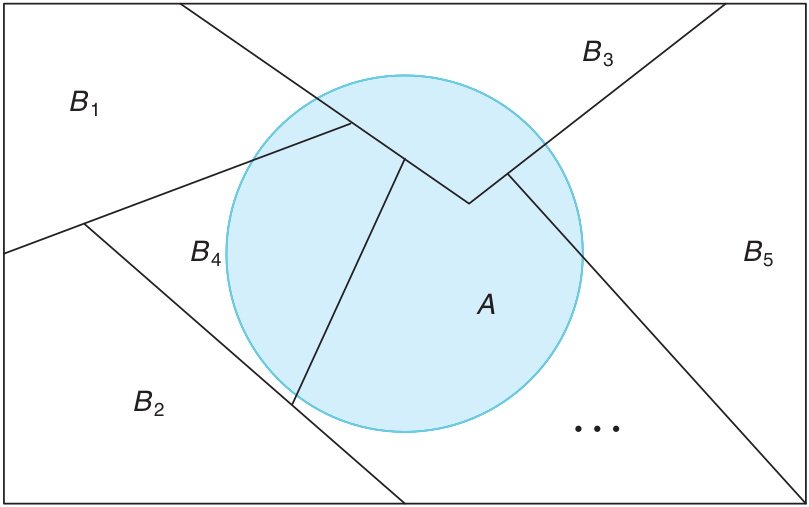
\includegraphics[width=0.35\textwidth]{venn_probabilidad_total}
    \end{center}
\end{frame}


\iffalse
\begin{frame}
    \frametitle{Regla / Teorema de Bayes}
    \begin{center}
        \begin{Huge}
            \emph{¡Éste es uno de los puntos más importantes de este curso!}
        \end{Huge}
    \end{center}
\end{frame}

\begin{frame}
    \frametitle{Reinterpretación ejemplo: bolsa con 4 pelotas}
    \begin{block}{Posibilidades}
        \begin{center}
            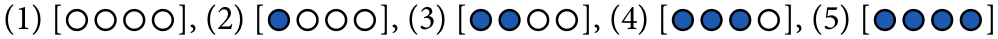
\includegraphics[height=0.05\textheight]{pelotas_todas}
        \end{center}
    \end{block}
    \begin{block}{Experimento -- datos}
        \begin{itemize}
            \item Se saca una pelota 3 veces con repetición:
        \end{itemize}
        \begin{center}
            
\includegraphics[height=0.04\textheight]{pelotas_datos}
        \end{center}
    \end{block}
    \begin{block}{Probabilidad -- grado de creencia}
        \begin{center}
            $\prob{
\includegraphics[height=0.05\textheight]{pelotas_conjetura} \mid
            
\includegraphics[height=0.04\textheight]{pelotas_datos}}$
        \end{center}
    \end{block}
\end{frame}

\begin{frame}
    \frametitle{Reinterpretación ejemplo: bolsa con 4 pelotas}
    \begin{center}
        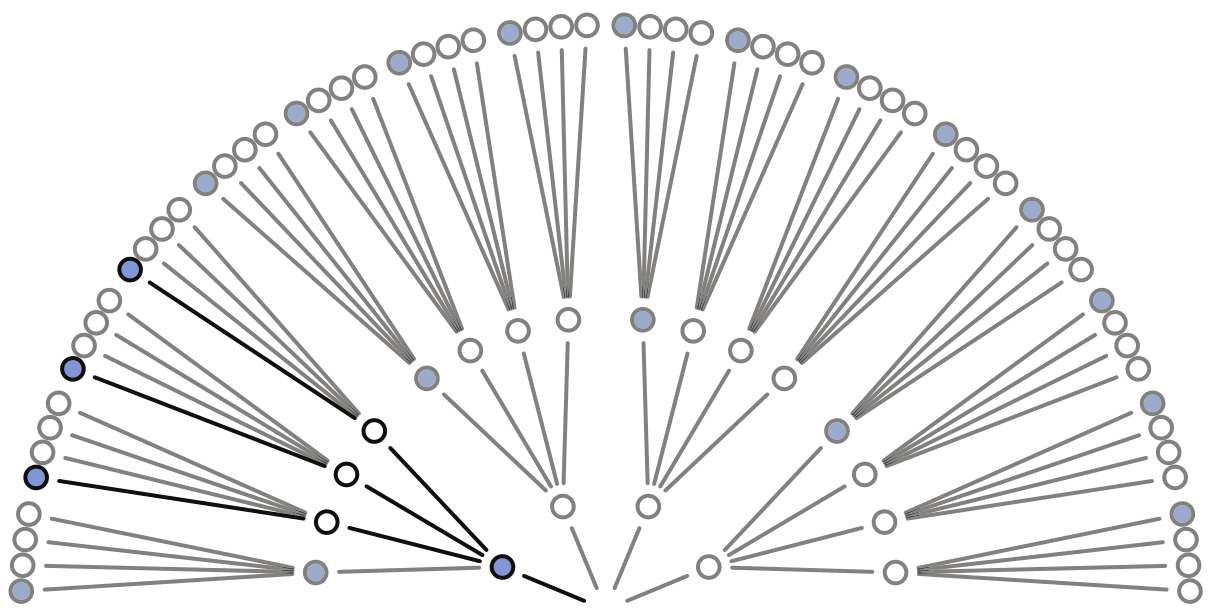
\includegraphics[height=0.513\textheight]{pelotas_arbol_4}
    \end{center}
    \begin{center}
        Espacio de eventos condicionales a ``hipótesis'' 
\includegraphics[height=0.05\textheight]{pelotas_conjetura}.
    \end{center}
\end{frame}

\begin{frame}
    \frametitle{Reinterpretación ejemplo: bolsa con 4 pelotas}
    \begin{center}
        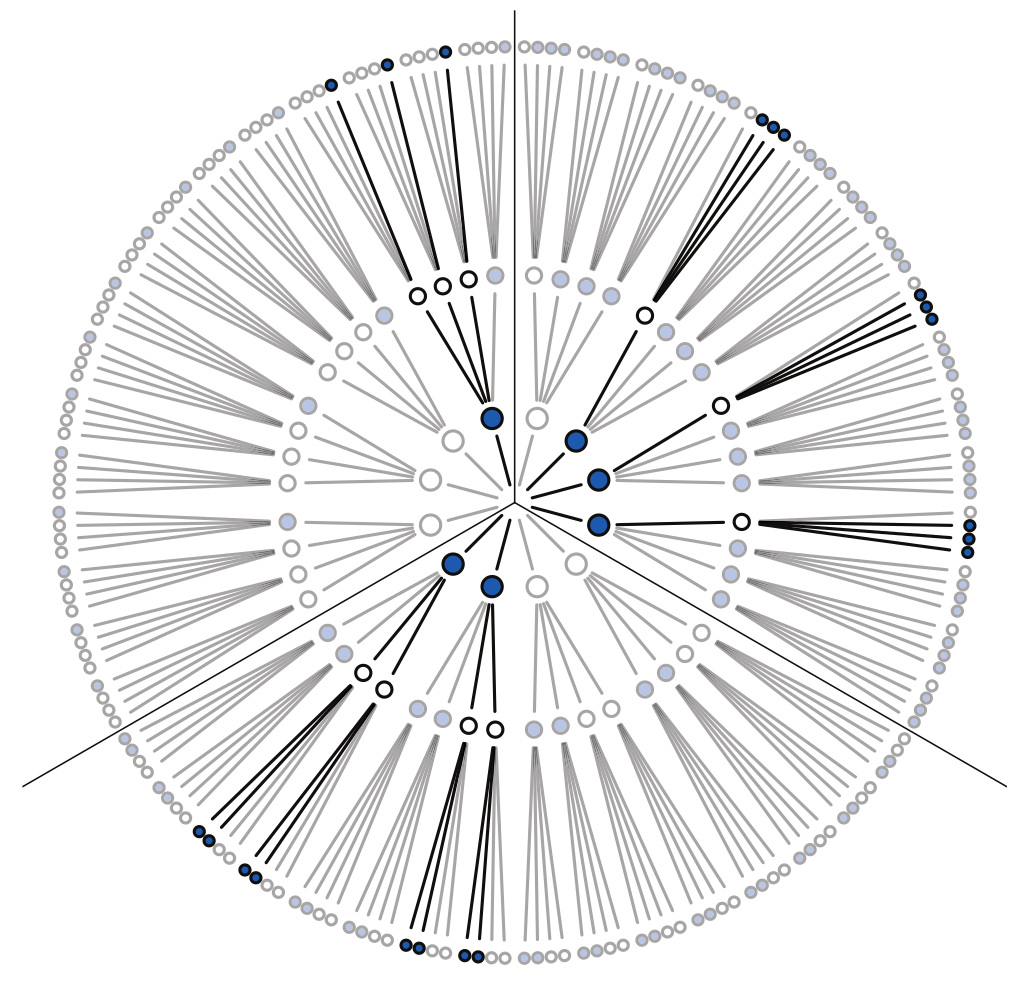
\includegraphics[height=0.8\textheight]{pelotas_todas_posibilidades}
    \end{center}
    \begin{center}
        Espacio de eventos condicionales a algunas ``hipótesis''.
    \end{center}
\end{frame}

\begin{frame}
    \frametitle{Reinterpretación ejemplo: bolsa con 4 pelotas}
    \begin{center}
        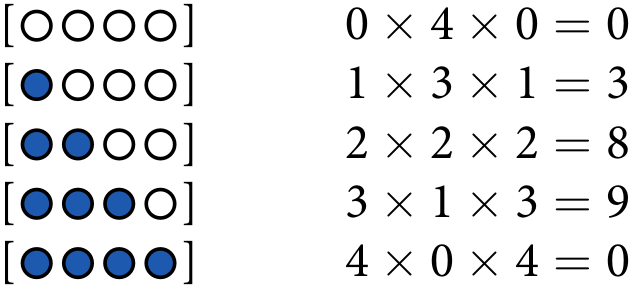
\includegraphics[height=0.4\textheight]{pelotas_conjeturas}
    \end{center}
    \begin{block}{Probabilidad -- grado de creencia}
        \begin{equation*}
            \prob{
\includegraphics[height=0.05\textheight]{pelotas_conjetura} \mid
            
\includegraphics[height=0.04\textheight]{pelotas_datos}} .
        \end{equation*}
    \end{block}
\end{frame}

\begin{frame}
    \frametitle{Reinterpretación ejemplo: bolsa con 4 pelotas}
    \begin{center}
        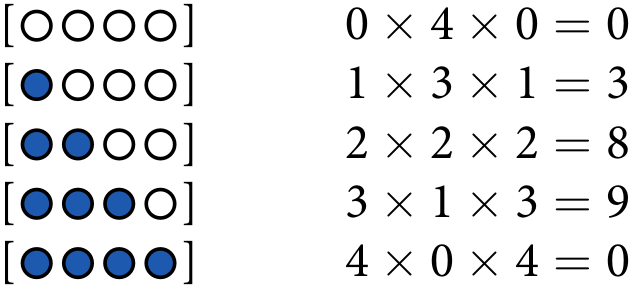
\includegraphics[height=0.4\textheight]{pelotas_conjeturas}
    \end{center}
    \begin{block}{Probabilidad -- grado de creencia}
        \begin{equation*}
            \prob{
\includegraphics[height=0.05\textheight]{pelotas_conjetura} \mid
            
\includegraphics[height=0.04\textheight]{pelotas_datos}} =
            \frac{\prob{
\includegraphics[height=0.04\textheight]{pelotas_datos} \mid
            
\includegraphics[height=0.05\textheight]{pelotas_conjetura}}
            \prob{
\includegraphics[height=0.05\textheight]{pelotas_conjetura}}}{\prob{
\includegraphics[height=0.04\textheight]{pelotas_datos}}} .
        \end{equation*}
    \end{block}
\end{frame}

\begin{frame}
    \frametitle{Reinterpretación ejemplo: bolsa con 4 pelotas}
    \begin{center}
        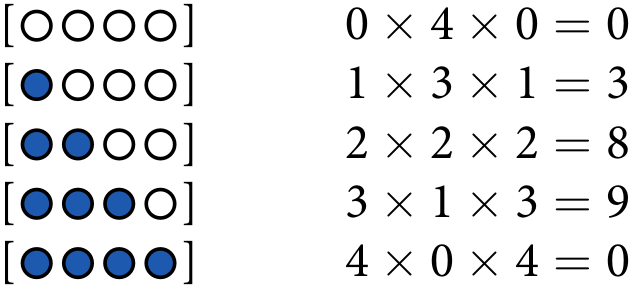
\includegraphics[height=0.4\textheight]{pelotas_conjeturas}
    \end{center}
    \begin{block}{Probabilidad -- grado de creencia}
        \begin{equation*}
            \prob{
\includegraphics[height=0.05\textheight]{pelotas_conjetura} \mid
            
\includegraphics[height=0.04\textheight]{pelotas_datos}} =
            \frac{\prob{
\includegraphics[height=0.04\textheight]{pelotas_datos} \mid
            
\includegraphics[height=0.05\textheight]{pelotas_conjetura}}
            \prob{
\includegraphics[height=0.05\textheight]{pelotas_conjetura}}}{
                \sum_{i = 0}^{4} \prob{
\includegraphics[height=0.04\textheight]{pelotas_datos} \mid c_{i}} \prob{c_{i}}} .
        \end{equation*}
    \end{block}
\end{frame}

\begin{frame}
    \frametitle{Reinterpretación ejemplo: bolsa con 4 pelotas}
    \begin{center}
        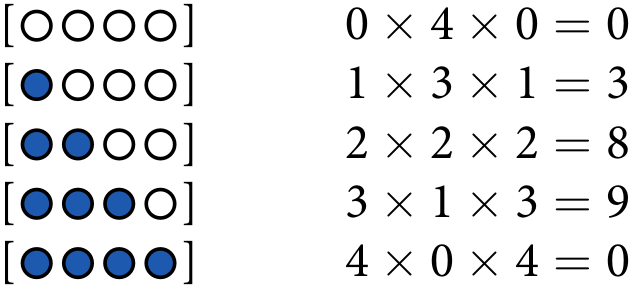
\includegraphics[height=0.4\textheight]{pelotas_conjeturas}
    \end{center}
    \begin{block}{Probabilidad -- supuesto}
        \begin{multline*}
            \prob{
\includegraphics[height=0.05\textheight]{pelotas_conjetura} \mid
            \includegraphics[height=0.04\textheight]{pelotas_datos}} =
            \frac{\frac{3}{64} \frac{1}{5}}{\frac{0}{64} \frac{1}{5} + \frac{3}{64} \frac{1}{5} + \frac{8}{64} \frac{1}{5} + \frac{9}{64} \frac{1}{5} + \frac{0}{64} \frac{1}{5}} \\
            = \frac{3 \frac{1}{5}}{0 \frac{1}{5} + 3 \frac{1}{5} + 8 \frac{1}{5} + 9 \frac{1}{5} + 0 \frac{1}{5}}
            = \frac{3}{20} = 0.15 .
        \end{multline*}
    \end{block}
\end{frame}

\begin{frame}
    \frametitle{Reinterpretación ejemplo: bolsa con 4 pelotas}
    \begin{center}
        \includegraphics[height=0.4\textheight]{pelotas_conjeturas}
    \end{center}
    \begin{block}{Probabilidad -- otro supuesto}
        \begin{equation*}
            \prob{\includegraphics[height=0.05\textheight]{pelotas_conjetura} \mid
            \includegraphics[height=0.04\textheight]{pelotas_datos}} =
            \frac{3 \frac{4}{16}}{0 \frac{1}{16} + 3 \frac{4}{16} + 8 \frac{6}{16} + 9 \frac{4}{16} + 0 \frac{1}{16}}
            = \frac{1}{8} = 0.125 .
        \end{equation*}
    \end{block}
\end{frame}

\begin{frame}
    \frametitle{Reinterpretación ejemplo: bolsa con 4 pelotas}
    \begin{center}
        \includegraphics[height=0.4\textheight]{pelotas_conjeturas}
    \end{center}
    \begin{block}{Probabilidad -- resultado como nuevo supuesto}
        \begin{equation*}
            \prob{\includegraphics[height=0.05\textheight]{pelotas_conjetura} \mid
            \includegraphics[height=0.04\textheight]{pelotas_datos}} =
            \frac{3 \frac{1}{5}}{0 \frac{1}{5} + 3 \frac{1}{5} + 8 \frac{1}{5} + 9 \frac{1}{5} + 0 \frac{1}{5}}
            = \frac{3}{20} = 0.15 .
        \end{equation*}
    \end{block}
\end{frame}

\begin{frame}
    \frametitle{Reinterpretación ejemplo: bolsa con 4 pelotas}
    \begin{center}
        Se saca una nueva pelota:
        \includegraphics[height=0.04\textheight]{pelotas_una}.
    \end{center}
    \begin{center}
        \includegraphics[height=0.4\textheight]{pelotas_nueva_cuenta}
    \end{center}
    \begin{block}{Probabilidad -- nueva pelota y anterior supuesto}
        \begin{multline*}
            \prob{\includegraphics[height=0.05\textheight]{pelotas_conjetura} \mid
            \includegraphics[height=0.035\textheight]{pelotas_una}} =
            \frac{\frac{1}{4} \frac{3}{20}}{\frac{0}{4} \frac{0}{20} + \frac{1}{4} \frac{3}{20} + \frac{2}{4} \frac{8}{20} + \frac{3}{4} \frac{9}{20} + \frac{4}{4} \frac{0}{20}} \\
            = \frac{1 \frac{3}{20}}{0 \frac{0}{20} + 1 \frac{3}{20} + 2 \frac{8}{20} + 3 \frac{9}{20} + 4 \frac{0}{20}}
            = \frac{3}{46} \approx 0.065 .
        \end{multline*}
    \end{block}
\end{frame}
\fi 



\begin{frame}
    \frametitle{Regla / Teorema de Bayes}
    \begin{block}{Actualización de estado de creencia}
        \begin{equation*}
            \underbrace{\prob{B \mid A}}_{\text{posterior}} = \frac{\overbrace{\prob{A \mid B}}^{\text{verosimilitud}} \overbrace{\prob{B}}^{\text{prior}}}{\underbrace{\prob{A}}_{\text{evidencia}}} .
        \end{equation*}
        \begin{itemize}
            \item $\prob{B}$ probabilidad a priori (\emph{prior}).
            \item $\prob{A \mid B}$ verosimilitud de $B$ (\emph{likelihood}).
            \item $\prob{A}$ evidencia.
            \item $\prob{B \mid A}$ probabilidad a posteriori (\emph{posterior}).
        \end{itemize}
    \end{block}

\end{frame}




\begin{frame}
    \frametitle{Regla / Teorema de Bayes}
    \begin{block}{Ejemplo mensajes Morse}
		Considere la transmisión de mensajes codificados mediante secuencias de `\textbf{.}' y `\textbf{\_}'. La ocurrencia de estos simbolos sucede en proporción de 3:4, por lo tanto:
$$P(\{. env\})=\frac{3}{7}\ y\ P(\{\_ env\})=\frac{4}{7} $$

Existen \textit{Interferencia}. Un `\textbf{.}' es erroneamente recibido como `\textbf{\_}' (\textbf{y viceversa}) con probabilidad $\frac{1}{8}$


\textbf{¿?} Al recibir un `\textbf{.}', ¿qué tan seguros podemos estar de que fue un `\textbf{.}' lo que se envió?
    \end{block}
\end{frame}

\begin{frame}

\end{frame}


\begin{frame}
\frametitle{Regla / Teorema de Bayes}

\begin{block}{Eventos disjuntos}
        \begin{itemize}
            \item $\bparens{B_{1}, \ldots, B_{n}}$ partición de $\Omega$:
                \begin{equation*}
                    \forall i, \prob{B_{i} \mid A} = \frac{\prob{A \mid B_{i}} \prob{B_{i}}}{\prob{A}}
                    =
                    \frac{\prob{A \mid B_{i}} \prob{B_{i}}}{\sum_{j = 1}^{n} \prob{A \mid B_{j}} \prob{B_{j}}} .
                \end{equation*}
        \end{itemize}
    \end{block}
\end{frame}

\begin{frame}
    \frametitle{Regla / Teorema de Bayes}
    \begin{block}{Ejemplo: examen}
        \begin{itemize}
            \item $\prob{\text{examen positivo} \mid \text{enfermedad}} = \frac{290}{10 + 290} = \frac{29}{30} \approx 0.97$.
            \item $\prob{\text{examen negativo} \mid \text{enfermedad}} = \frac{10}{10 + 290} = \frac{1}{30} \approx 0.03$.
            \item $\prob{\text{examen positivo} \mid \text{no enfermedad}} = \frac{10000}{10000 + 200000} = \frac{1}{21} \approx 0.05$.
            \item $\prob{\text{examen negativo} \mid \text{no enfermedad}} = \frac{200000}{10000 + 200000} = \frac{20}{21} \approx 0.95$.
        \end{itemize}
    \end{block}
    \begin{center}
        \begin{tabular}{c|cc}
            & Enfermedad & No Enfermedad \\
            \hline
            Examen Positivo & 290 & 10000 \\
            Examen Negativo & 10 & 200000 \\
        \end{tabular}
    \end{center}
    \begin{block}{Pregunta}
        \begin{itemize}
            \item ¿$\prob{\text{enfermedad} \mid \text{examen positivo}}$?
        \end{itemize}
    \end{block}
\end{frame}

\begin{frame}
    \frametitle{Regla / Teorema de Bayes}
    \begin{block}{Ejemplo: examen}
        \begin{itemize}
            \item $\prob{\text{examen positivo} \mid \text{enfermedad}} = 0.97$.
            \item $\prob{\text{examen negativo} \mid \text{enfermedad}} = 0.03$.
            \item $\prob{\text{examen positivo} \mid \text{no enfermedad}} = 0.05$.
            \item $\prob{\text{examen negativo} \mid \text{no enfermedad}} = 0.95$.
        \end{itemize}
    \end{block}
    \begin{block}{Pregunta}
        \begin{itemize}
            \item ¿$\prob{\text{enfermedad} \mid \text{examen positivo}}$?
        \end{itemize}
    \end{block}
\end{frame}

\begin{frame}
    \frametitle{Regla / Teorema de Bayes}
    \begin{block}{Ejemplo: alarma, parte 1}
        \begin{itemize}
            \item Cristián maneja desde Valparaíso a San Felipe por trabajo.
            \item Mientras trabaja, recibe una llamada de sus vecinos que le dicen que está sonando la alarma de su casa.
            \item ¿Probabilidad de que haya entrado un ladrón en su casa?
        \end{itemize}
    \end{block}
    \begin{block}{Ejemplo: alarma, parte 2}
        \begin{itemize}
            \item Mientras maneja de vuelta a su casa para ver qué sucedió, escucha en la radio que hubo un pequeño temblor cerca de su casa en Valparaíso.
            \item Se siente aliviado: ``probablemente fue el temblor el que activó la alarma''.
            \item ¿Probabilidad de que haya entrado un ladrón en su casa?
        \end{itemize}
    \end{block}
\end{frame}

\begin{frame}
    \frametitle{Regla / Teorema de Bayes -- alarma}
    \begin{block}{Supuestos}
        \begin{itemize}
            \item Ladrón cada tres años: $\prob{L} = 0.001$.
            \item Terremoto cada tres años: $\prob{T} = 0.001$.
            \item Ladrón independiente de terremoto: $\prob{L, T} = \prob{L} \prob{T}$.
            \item Alarma suena:
                \begin{itemize}
                    \item $99\%$ de las veces que hay un ladrón.
                    \item $1\%$ de las veces que hay un terremoto.
                    \item Otros eventos disparan la alarma con frecuencia $0.001$.
                \end{itemize}
            \item Vecinos nunca llaman si la alarma no suena: $\prob{V \mid A^{c}} = 0$.
            \item Radio no anuncia terremotos que no ocurrieron: $\prob{R \mid T^{c}} = 0$.
        \end{itemize}
    \end{block}
\end{frame}

\begin{frame}
    \frametitle{Regla / Teorema de Bayes -- alarma}
    \begin{block}{Supuestos de alarma}
        \begin{itemize}
            \item $\prob{A^{c} \mid L, T} = \parens{1 - 0.001} \parens{1 - 0.99} \parens{1 - 0.01} = 0.0098901$.
            \item $\prob{A^{c} \mid L^{c}, T} = \parens{1 - 0.001} \parens{1 - 0.01} = 0.98901$.
            \item $\prob{A^{c} \mid L, T^{c}} = \parens{1 - 0.001} \parens{1 - 0.99} = 0.00999$.
            \item $\prob{A^{c} \mid L^{c}, T^{c}} = 1 - 0.001 = 0.999$.
            \item $\prob{A \mid L, T} = 1 - \parens{1 - 0.001} \parens{1 - 0.99} \parens{1 - 0.01} = 0.9901099$.
            \item $\prob{A \mid L^{c}, T} = 1 - \parens{1 - 0.001} \parens{1 - 0.01} = 0.01099$.
            \item $\prob{A \mid L, T^{c}} = 1 - \parens{1 - 0.001} \parens{1 - 0.99} = 0.99001$.
            \item $\prob{A \mid L^{c}, T^{c}} = 0.001$.
        \end{itemize}
    \end{block}
\end{frame}

\begin{frame}
    \frametitle{Regla / Teorema de Bayes -- alarma}
    \begin{block}{Posterior}
        \begin{itemize}
            \item $\prob{L, T \mid A} = \frac{1}{\prob{A}} \prob{A \mid L, T} \prob{L} \prob{T}$.
            \item $\prob{L^{c}, T \mid A} = \frac{1}{\prob{A}} \prob{A \mid L^{c}, T} \prob{L^{c}} \prob{T}$.
            \item $\prob{L, T^{c} \mid A} = \frac{1}{\prob{A}} \prob{A \mid L, T^{c}} \prob{L} \prob{T^{c}}$.
            \item $\prob{L^{c}, T^{c} \mid A} = \frac{1}{\prob{A}} \prob{A \mid L^{c}, T^{c}} \prob{L^{c}} \prob{T^{c}}$.
        \end{itemize}
    \end{block}
    \begin{block}{Posterior -- caso 1}
        \begin{itemize}
            \item $\prob{L, T \mid A}
                = 0.9901099 \times 0.001 \times 0.001 \frac{1}{\prob{A}} = 9.9 \times 10^{-7} \frac{1}{\prob{A}}$.
            \item $\prob{L^{c}, T \mid A}
                = 0.01099 \times 0.999 \times 0.001 \frac{1}{\prob{A}} = 0.000010979 \frac{1}{\prob{A}}$.
            \item $\prob{L, T^{c} \mid A}
                = 0.99001 \times 0.001 \times 0.999 \frac{1}{\prob{A}} = 0.000989 \frac{1}{\prob{A}}$.
            \item $\prob{L^{c}, T^{c} \mid A}
                = 0.001 \times 0.999 \times 0.999 \frac{1}{\prob{A}} = 0.000998 \frac{1}{\prob{A}}$.
            \item $\prob{A} = \text{Suma} = 0.002$.
        \end{itemize}
    \end{block}
\end{frame}

\begin{frame}
    \frametitle{Regla / Teorema de Bayes -- alarma}
    \begin{block}{Ejemplo: alarma, parte 1}
        \begin{itemize}
            \item Cristián maneja desde Valparaíso a San Felipe por trabajo.
            \item Mientras trabaja, recibe una llamada de sus vecinos que le dicen que está sonando la alarma de su casa.
            \item ¿Probabilidad de que haya entrado un ladrón en su casa?
        \end{itemize}
    \end{block}
    \begin{block}{Posterior -- caso 1}
        \begin{itemize}
            \item $\prob{L, T \mid A} = 0.0005$.
            \item $\prob{L^{c}, T \mid A} = 0.0055$.
            \item $\prob{L, T^{c} \mid A} = 0.4947$.
            \item $\prob{L^{c}, T^{c} \mid A} = 0.4993$.
            \item Respuesta: $\prob{L \mid A} = \prob{L, T \mid A} + \prob{L, T^{c} \mid A} \approx 0.495$.
        \end{itemize}
    \end{block}
\end{frame}

\begin{frame}
    \frametitle{Regla / Teorema de Bayes -- alarma}
    \begin{block}{Ejemplo: alarma, parte 2}
        \begin{itemize}
            \item Mientras maneja de vuelta a su casa para ver qué sucedió, escucha en la radio que hubo un pequeño temblor cerca de su casa en Valparaíso.
            \item Se siente aliviado: ``probablemente fue el temblor el que activó la alarma''.
            \item ¿Probabilidad de que haya entrado un ladrón en su casa?
        \end{itemize}
    \end{block}
    \begin{block}{Posterior -- caso 2}
        \begin{itemize}
            \item $\prob{L, T \mid A} = 0.0005$.
            \item $\prob{L^{c}, T \mid A} = 0.0055$.
            \item $\prob{L, T^{c} \mid A} = 0.4947$.
            \item $\prob{L^{c}, T^{c} \mid A} = 0.4993$.
            \item Respuesta: $\prob{L \mid A, T} = \frac{\prob{L, T \mid A}}{\prob{T \mid A}}
                = \frac{\prob{L, T \mid A}}{\prob{L, T \mid A} + \prob{L^{c}, T \mid A}}
                = \frac{0.0005}{0.0005 + 0.0055} \approx 0.08$.
        \end{itemize}
    \end{block}
\end{frame}

\begin{frame}
    \frametitle{Regla / Teorema de Bayes -- videos recomendados}
    \begin{block}{Probabilidades y teorema de Bayes}
        \begin{itemize}
            \item \url{https://www.youtube.com/watch?v=HZGCoVF3YvM}.
            \item \url{https://www.youtube.com/watch?v=U_85TaXbeIo}.
        \end{itemize}
    \end{block}
    \begin{block}{Paradoja del examen médico}
        \begin{itemize}
            \item \url{https://www.youtube.com/watch?v=lG4VkPoG3ko}.
        \end{itemize}
    \end{block}
\end{frame}

\begin{frame}
    \frametitle{Ejemplo: mensaje por canal ruidoso}
    \begin{block}{Canal ruidoso}
        \begin{itemize}
            \item Probabilidad de cambiar un bit: $f$.
        \end{itemize}
    \end{block}
    \begin{block}{Código de repetición}
        \begin{itemize}
            \item Si se quiere comunicar 1, se envía 111.
            \item Si se quiere comunicar 0, se envía 000.
        \end{itemize}
    \end{block}
    \begin{block}{Ejemplo}
        \begin{itemize}
            \item Se recibe mensaje 000 001 111 000 010 111 000.
            \item ¿Cuál es el mensaje original?
        \end{itemize}
    \end{block}
\end{frame}

\begin{frame}
    \frametitle{Ejemplo: mensaje por canal ruidoso}
    \begin{block}{Ejemplo}
        \begin{itemize}
            \item Se recibe mensaje 000 001 111 000 010 111 000.
            \item ¿Cuál es el mensaje original?
        \end{itemize}
    \end{block}
    \begin{block}{Bayes}
        \begin{equation*}
            \prob{\text{bit} \mid r_{1} r_{2} r_{3}} = \frac{\prob{r_{1} r_{2} r_{3} \mid \text{bit}} \prob{\text{bit}}}{\prob{r_{1} r_{2} r_{3}}} .
        \end{equation*}
    \end{block}
\end{frame}

\begin{frame}
    \frametitle{Ejemplo: mensaje por canal ruidoso}
    \begin{block}{Ruido al comunicar un bit por el canal}
        \begin{itemize}
            \item $\prob{0 \mid 0} = 1 - f$.
            \item $\prob{1 \mid 0} = f$.
            \item $\prob{0 \mid 1} = f$.
            \item $\prob{1 \mid 1} = 1 - f$.
        \end{itemize}
    \end{block}
    \begin{block}{Tres bits recibidos}
        \begin{itemize}
            \item $\prob{000 \mid 0} = \parens{1 - f}^{3}$.
            \item $\prob{001 \mid 0} = \parens{1 - f}^{2} f$.
            \item $\prob{011 \mid 0} = \parens{1 - f} f^{2}$.
            \item $\prob{111 \mid 0} = f^{3}$.
        \end{itemize}
    \end{block}
\end{frame}

\begin{frame}
    \frametitle{Ejemplo: mensaje por canal ruidoso}
    \begin{center}
        \begin{tabular}{cccc}
            Recibido & Enviado & Original & \\
            \hline
            000 & 000 & 0 & $\prob{000 \mid 0} = \parens{1 - f}^{3}$ \\
            000 & 111 & 1 & $\prob{000 \mid 1} = f^{3}$ \\
            001 & 000 & 0 & $\prob{001 \mid 0} = \parens{1 - f}^{2} f$ \\
            001 & 111 & 1 & $\prob{001 \mid 1} = \parens{1 - f} f^{2}$ \\
            010 & 000 & 0 & $\prob{010 \mid 0} = \parens{1 - f}^{2} f$ \\
            010 & 111 & 1 & $\prob{010 \mid 1} = \parens{1 - f} f^{2}$ \\
            100 & 000 & 0 & $\prob{100 \mid 0} = \parens{1 - f}^{2} f$ \\
            100 & 111 & 1 & $\prob{100 \mid 1} = \parens{1 - f} f^{2}$ \\
            011 & 000 & 0 & $\prob{011 \mid 0} = \parens{1 - f} f^{2}$ \\
            011 & 111 & 1 & $\prob{011 \mid 1} = \parens{1 - f}^{2} f$ \\
            101 & 000 & 0 & $\prob{101 \mid 0} = \parens{1 - f} f^{2}$ \\
            101 & 111 & 1 & $\prob{101 \mid 1} = \parens{1 - f}^{2} f$ \\
            110 & 000 & 0 & $\prob{110 \mid 0} = \parens{1 - f} f^{2}$ \\
            110 & 111 & 1 & $\prob{110 \mid 1} = \parens{1 - f}^{2} f$ \\
            111 & 000 & 0 & $\prob{111 \mid 0} = f^{3}$ \\
            111 & 111 & 1 & $\prob{111 \mid 1} = \parens{1 - f}^{3}$
        \end{tabular}
    \end{center}
\end{frame}

\begin{frame}
    \frametitle{Ejemplo: mensaje por canal ruidoso}
    \begin{block}{Ejemplo}
        \begin{itemize}
            \item Se recibe mensaje 000 001 111 000 010 111 000.
            \item ¿Cuál es el mensaje original?
        \end{itemize}
    \end{block}
    \begin{block}{Posterior}
        \begin{itemize}
            \item Elegimos el bit con mayor posterior.
            \item Calculamos la razón entre bit 0 y 1:
                \begin{equation*}
                    \text{razón} \parens{r_{1} r_{2} r_{3}} = \frac{\prob{0 \mid r_{1} r_{2} r_{3}}}{\prob{1 \mid r_{1} r_{2} r_{3}}} =
                    \frac{\frac{\prob{r_{1} r_{2} r_{3} \mid 0} \prob{0}}{\prob{r_{1} r_{2} r_{3}}}}{\frac{\prob{r_{1} r_{2} r_{3} \mid 1} \prob{1}}{\prob{r_{1} r_{2} r_{3}}}}
                    = \frac{\prob{r_{1} r_{2} r_{3} \mid 0} \prob{0}}{\prob{r_{1} r_{2} r_{3} \mid 1} \prob{1}} .
                \end{equation*}
            \item $\prob{0}$ y $\prob{1}$ no dependen del mensaje.
            \item Necesitamos solo la razón de la verosimilitud $\frac{\prob{r_{1} r_{2} r_{3} \mid 0}}{\prob{r_{1} r_{2} r_{3} \mid 1}}$.
        \end{itemize}
    \end{block}
\end{frame}

\begin{frame}
\frametitle{Ejemplo: mensaje por canal ruidoso}
\begin{itemize}
\item Ejemplo:
                \begin{equation*}
                    \text{razón} \parens{000}
                    = \frac{\prob{000 \mid 0}}{\prob{000 \mid 1}} \frac{\prob{0}}{\prob{1}}
                    = \frac{\parens{1 - f}^{3}}{f^{3}}
                    \frac{\prob{0}}{\prob{1}}
                    = \gamma^{3} \frac{\prob{0}}{\prob{1}} .
                \end{equation*}
\end{itemize}

\end{frame}

\begin{frame}
    \frametitle{Ejemplo: mensaje por canal ruidoso}
    \begin{block}{Ejemplo}
        \begin{itemize}
            \item Se recibe mensaje 000 001 111 000 010 111 000.
            \item ¿Cuál es el mensaje original?
        \end{itemize}
    \end{block}
    \begin{center}
        \begin{tabular}{ccc}
            Bits recibidos & Razón de verosimilitud & Respuesta \\
            \hline
            000 & $\gamma^{3}$ & 0 \\
            001 & $\gamma$ & 0 \\
            010 & $\gamma$ & 0 \\
            100 & $\gamma$ & 0 \\
            011 & $\gamma^{-1}$ & 1 \\
            101 & $\gamma^{-1}$ & 1 \\
            110 & $\gamma^{-1}$ & 1 \\
            111 & $\gamma^{-3}$ & 1 \\
        \end{tabular}
    \end{center}
    \begin{block}{Respuesta}
        \begin{itemize}
            \item Si $\prob{0} = \prob{1}$, el mensaje recuperado es 0010010.
        \end{itemize}
    \end{block}
\end{frame}

\begin{frame}
    \frametitle{Ejemplo: mensaje por canal ruidoso}
    \begin{center}
        \includegraphics[width=\textwidth]{decoder}
    \end{center}
\end{frame}

\begin{frame}
    \frametitle{Problema de Monty Hall}
    \begin{block}{Funcionamiento del juego}
        \begin{itemize}
            \item Hay tres puertas, etiquetadas como $1$, $2$ y $3$.
            \item Hay un premio, atrás de una sola de las puertas.
            \item Se selecciona una puerta donde se cree que se encuentra el premio.
            \item En vez de abrir esa puerta, el presentador abre una de las otras dos puertas, de manera de abrir una puerta que no tiene el premio.
            \item Se ofrece la alternativa de quedarse con la puerta seleccionada, o cambiarse a la otra que quedó cerrada.
            \item Finalmente, se abren todas las puertas y se recibe lo que haya detrás de la puerta seleccionada.
        \end{itemize}
    \end{block}
    \begin{center}
        \includegraphics[height=0.24\textheight]{monty-hall-problem}
    \end{center}
\end{frame}

\begin{frame}
    \frametitle{Monty Hall -- Tres puertas, reglas normales}
    \begin{block}{Pregunta de ejemplo}
        \begin{itemize}
            \item Participante elige puerta $1$ primero.
            \item Presentador abre puerta $3$, mostrando que no hay nada en esa puerta.
            \item El participante debería:
                \begin{itemize}
                    \item Quedarse con la puerta $1$.
                    \item Cambiar a la puerta $2$.
                    \item No hay diferencia si elige puerta $1$ o $2$.
                \end{itemize}
        \end{itemize}
    \end{block}
    \begin{center}
        \includegraphics[height=0.27\textheight]{monty-hall-problem}
    \end{center}
\end{frame}

\begin{frame}
    \frametitle{Monty Hall -- Tres puertas, escenario temblor}
    \begin{block}{Cambio en el juego}
        \begin{itemize}
            \item Cuando el presentador se dispone a abrir una de las puertas, hay un temblor y se abre la misma puerta $3$, que no tiene el premio.
            \item El presentador dice ``ah, bueno, ahora que se abrió una puerta, sigamos adelante''.
            \item Se ofrece la alternativa de quedarse con la puerta seleccionada, o cambiarse a la otra que quedó cerrada.
            \item Finalmente, se abren todas las puertas y se recibe lo que haya detrás de la puerta seleccionada.
        \end{itemize}
    \end{block}
    \begin{block}{El participante debería}
        \begin{itemize}
            \item Quedarse con la puerta $1$.
            \item Cambiar a la puerta $2$.
            \item No hay diferencia si elige puerta $1$ o $2$.
        \end{itemize}
    \end{block}
\end{frame}

\begin{frame}
    \frametitle{Monty Hall -- Ejercicio}
    \begin{block}{Muchas puertas}
        \begin{itemize}
            \item En vez de $3$ puertas, hay un millón de ellas.
            \item Luego de seleccionar la primera puerta, el presentador abre $999998$ puertas que no tienen el premio atrás, dejando solo dos puertas cerradas.
            \item Por ejemplo, participante eligió puerta $1$ y luego quedan cerradas solo las puertas $1$ y $234598$.
            \item ¿Dónde cree que está el premio?
        \end{itemize}
    \end{block}
    \begin{alertblock}{Regla general (Steve Gull)}
        \begin{itemize}
            \item \emph{Siempre escribir la probabilidad de todo.}
        \end{itemize}
    \end{alertblock}
\end{frame}

\begin{frame}
    \frametitle{Interpretación probabilidades -- UK Met Office}
    \begin{block}{}
        \begin{itemize}
            \item
                Supongamos que la oficina dice que la probabilidad de llover mañana en
                tu región es de $80\%$.
                No están diciendo que lloverá en un $80\%$ del área de terreno de tu región,
                y no lloverá en el restante $20\%$. Tampoco están diciendo que lloverá un $80\%$ del tiempo.
                Lo que están diciendo es que hay una posibilidad de un $80\%$ de que llueva
                en cualquier lugar de la región, como tu jardín.
            \item
                Un pronóstico de $80\%$ de posibilidad de lluvia en tu región debería significar más o menos
                que, en alrededor de un $80\%$ de los días en que las condiciones climáticas son como las de mañana,
                se experimentará lluvia donde estás.
            \item
                Si no llueve en tu jardín mañana, entonces el pronóstico de $80\%$ no está equivocado,
                porque no djo que la lluvia era segura. Pero si miras a lo largo de los días, en que
                la oficina dijo que la probabilidad de lluvia era un $80\%$, deberías esperar que
                haya llovido en alrededor de un $80\%$ de ellos.
        \end{itemize}
    \end{block}
    %\scriptsize{\url{https://www.tiktok.com/@metoffice/video/6933249547871227141}}
    \url{https://www.tiktok.com/@metoffice/video/6933249547871227141}
\end{frame}

\iffalse
\begin{frame}[allowframebreaks, noframenumbering]
\frametitle<presentation>{References}
\printbibliography
%\bibliographystyle{apalike}
\end{frame}
\fi

\end{document}
